% !TEX program = xelatex
\documentclass{ustbthesis}


\usepackage[backend=biber,
style=gb7714-2015,%utf8,
    sortcites=true,autocite=inline,autopunct=true,hyperref=true,  
    natbib
    ]{biblatex}

\hypersetup{hidelinks,colorlinks=false,citecolor=black}
\addbibresource{myrefs.bib}
%\usepackage[numbers,super]{gbt7714}
%\newcommand{\upcite}[1]{\textsuperscript{\textsuperscript{\cite{#1}}}}
%\bibliography{myrefs}


\usepackage{tabularx}
\usepackage{amsmath}
\usepackage{amssymb}
\usepackage[labelfont=bf,textfont=bf,font=small]{subfig}
\newcommand{\figref}[1]{~\ref{#1}~}
\newcommand{\tabref}[1]{~\ref{#1}~}

\newcolumntype{P}[1]{>{\centering\arraybackslash}p{#1}}
%\addbibresource{myrefs.bib}
%%%%%%%%%%%%%%%%%%%%%%%%%%%封面信息%%%%%%%%%%%%%%%%%%%%%%%%%%%%%%%%%%
\Author{程立夫}
\EnglishAuthor{Lifu Cheng}
\Title{基于多智能体强化学习的建筑群节能控制策略及可视化研发}
\EnglishTitle{Energy-Saving Control Strategy and Visualization Development for Building Clusters Based on Multi-Agent Reinforcement Learning}
\Date{2026年12月}
\EnglishDate{Dec, 2026}
\College{数理学院}
\EnglishCollege{School of Mathematics and Physics}
\Address{海淀区学院路30号}
\EnglishAddress{30 Xueyuan Road, Haidian District}
\Affiliation{北京科技大学}
\EnglishAffiliation{University of Science and Technology Beijing}
\Postcode{100083}
\City{北京}
\EnglishCity{Beijing}
\Country{中国}
\EnglishCountry{P.R.CHINA}
\StudentCode{M202440085}
\Major{软件工程}
\EnglishMajor{Software Engineering}
\Direction{人工智能方向}
\EnglishDirection{Artificial Intelligence}
\Supervisor{段世红}
\EnglishSupervisor{Shihong Duan}
\DegreeType{学术型}
\EnglishDegreeType{Science}
\CLCNumber{TP319}
\UDCNumber{620}
\UniversityCode{10008}
\UniversityLogoFile{images/ustb.png}
\SecurityLevel{公开}
\SubmissionDate{2026年12月}
\EnglishSubmissionDate{Dec, 2026}
%%%%%%%%%%%%%%%%%%%%%%%%%%%封面信息%%%%%%%%%%%%%%%%%%%%%%%%%%%%%%%%%%
\begin{document}

\TitlePage

\SecondPage

\ThirdPage

\pagestyle{fancy}

%% 中英文摘要
\begin{ChineseAbstract}

建筑群能源系统同时受到天气、负荷、能源价格、分布式能源和用户舒适性需求的影响，具有强耦合、强不确定性和多目标特征。传统固定规则控制适应性不足，模型预测控制依赖精确模型并具有较高计算成本，而纯多智能体强化学习又容易面临样本效率低、训练不稳定和安全约束难以满足等问题。CityLearn为建筑群需求侧管理提供了统一的仿真环境、数据接口和评价指标，为控制策略的公平比较与可复现研究提供了基础。

在提出改进之前，现有方法仍面临三类核心难题：其一，以CHESCA为代表的规则与预测混合基线虽稳健可解释，但参数相对静态，难以及时适应负荷漂移、设备老化与极端天气；其二，纯多智能体强化学习虽具有长期优化潜力，却在小样本、非平稳环境和安全约束下难以稳定落地；其三，建筑群节能控制实验普遍存在难管理、难理解与难工程化使用的问题，算法配置、KPI对比与决策过程缺少统一可视化支撑。

针对上述难题，本文面向CityLearn建筑群能源管理场景，提出基于社区分层协调控制与残差多智能体强化学习的混合节能控制方法（CHESCA-ResMARL），并实现配套可视化管理平台。首先，系统梳理并复现CHESCA分层控制链路，建立标准化状态、动作与KPI模型；其次，在CHESCA基准动作之上叠加轻量级多智能体残差策略，通过动作掩码与安全投影实现“先验保安全、学习求增益”；再次，设计融合电价电费、制冷电费、电池套利、电池损耗与热舒适性的多目标奖励，并以消融、多种子与多场景实验评价方法有效性；最后，依托Vue、Spring Boot、MySQL与Python算法组件，贯通数据管理、算法配置、仿真任务、KPI分析与决策轨迹追踪。

项目已经完成CityLearn数据集构建、CHESCA基线评估、残差多智能体训练入口、动作安全约束、KPI导出和前后端可视化平台。实验结果表明，混合策略在保证舒适度的前提下实现了成本、碳排放、峰值与爬坡等多项指标的协同优化。本文的研究可为建筑群需求侧响应、低碳运行控制和智能能源管理系统的工程化应用提供参考。

\ChineseKeywords{建筑群节能；CityLearn；多智能体强化学习；残差强化学习；CHESCA；可视化管理}
\end{ChineseAbstract}

\begin{EnglishAbstract}

Building energy systems are affected by weather, demand, energy prices, distributed energy resources, and occupant comfort requirements. They therefore exhibit strong coupling, uncertainty, and multiple conflicting objectives. Fixed-rule control lacks adaptability, model predictive control relies on accurate models and high computational cost, while pure multi-agent reinforcement learning often suffers from low sample efficiency, training instability, and difficulty in satisfying safety constraints. CityLearn provides a standardized simulation environment, data interface, and evaluation metrics for building-community demand-side management, enabling reproducible and fair comparisons of control strategies.

Before the proposed improvements, existing approaches still face three core challenges. First, rule-and-prediction baselines such as CHESCA are robust and interpretable, yet relatively static and slow to adapt to load drift, equipment aging, and extreme weather. Second, pure multi-agent reinforcement learning has long-horizon optimization potential, but is difficult to deploy stably under limited samples, non-stationary environments, and hard safety constraints. Third, building-community energy-control experiments are commonly hard to manage, hard to interpret, and hard to engineer into usable systems, lacking unified support for algorithm configuration, KPI comparison, and decision tracing.

To address these challenges, this thesis investigates a hybrid energy-saving control method based on community hierarchical coordination and residual multi-agent reinforcement learning (CHESCA-ResMARL) for the CityLearn scenario, and develops an accompanying visualization management platform. First, the CHESCA hierarchical control pipeline is systematically reviewed and reproduced, and standardized state, action, and KPI models are established. Second, lightweight multi-agent residual policies are superimposed on CHESCA baseline actions, with action masks and safety projection realizing ``prior for safety, learning for gain''. Third, a multi-objective reward combining electricity cost, cooling cost, battery arbitrage, battery degradation, and thermal comfort is designed, and ablation, multi-seed, and cross-scenario evaluations are used to assess effectiveness. Finally, a visualization platform based on Vue, Spring Boot, MySQL, and Python algorithm services covers data management, algorithm configuration, simulation tasks, KPI analysis, and decision-trace inspection.

The current project has implemented CityLearn dataset construction, CHESCA baseline evaluation, a residual multi-agent training entry point, action safety constraints, KPI export, and a complete front-end/back-end visualization platform. Experimental results show that the hybrid strategy achieves coordinated optimization across cost, carbon emissions, peak load, and ramping while maintaining occupant comfort. This work may provide a reference for building-community demand response, low-carbon operation control, and engineering-oriented intelligent energy management systems.

\EnglishKeywords{building energy saving; CityLearn; multi-agent reinforcement learning; residual reinforcement learning; CHESCA; visualization management}
\end{EnglishAbstract}

%% 目录
\tableofcontents

\mainmatter
\pagenumbering{arabic}\setcounter{page}{1}
\pagestyle{fancy}

\chapter{引言}
\section{研究背景与意义}
建筑运行能耗长期居高不下。国际能源署在《Energy Efficiency 2023》中指出，建筑运行用能约占全球终端用能的三分之一，其中暖通空调与生活热水占据主要份额\cite{iea2023}。单栋建筑的节能控制相对简单，通过主机调节与定时策略即可取得成效；然而对于由多栋异构建筑组成的社区，问题显著复杂化：暖通、热水储能、电池与光伏等多种设备相互耦合，共用同一配电馈线、同一套分时电价与碳强度曲线。若A楼在高电价时段放电而B楼恰好在充电，社区总峰值反而可能被推高。这种耦合特性决定了建筑群控制并非单机回路的简单叠加，而是一个多智能体、多目标、部分可观测的序贯决策问题。

实际工程中的矛盾主要集中在四个方面。第一，经济性目标要求将负荷转移至电价低谷时段，而电网友好目标要求削峰并抑制爬坡，二者的最优工作点往往相互错开；第二，低碳运行希望在光伏大发、碳强度较低的时段多用电，这与实时电价的引导方向并不总是一致；第三，设备利用率与室内舒适度之间存在固有权衡，设备多运行一分、室温多偏离一分，效率与舒适便开始冲突；第四，中央协调器虽在理论上可获取全局信息，但现场通信、隐私与计算延迟等约束使完全集中式决策难以实现。因此，难点不仅在于寻得一个低能耗动作，更在于不确定性、异构性与安全约束并存的条件下，给出一个可解释、可落地的折中方案。

工程实践中应用最广泛的仍是规则控制（Rule-Based Control, RBC）与PID控制。基于运维经验的规则直观可靠、部署迅速，但参数一经固定，便难以适应次日电价走势与碳强度变化。模型预测控制（MPC）将约束写入滚动优化，控制效果良好\cite{mps2018,drgona2020mpc}；然而一旦模型失准，或建筑数量增多、设备类型复杂化，混合整数规划的求解规模迅速上升，在线运行面临较大计算压力。开题阶段梳理的BOPTEST框架为这类策略提供了高保真仿真与标准化测试用例，并以容器化部署和RESTful API支持MPC等先进策略的快速部署与评估\cite{boptest2021}；但其依赖精确模型、部署成本较高的特点意味着并非所有楼宇模型均可直接套用，这正是后文将MARL封装为易用闭环平台的动因之一。

强化学习提供了另一条技术路线：不依赖完整机理模型，通过与环境交互试错来获取长期回报。DQN将值函数引入神经网络\cite{mnih2015}，DDPG与SAC处理连续动作空间\cite{ddpg2016,haarnoja2018}，PPO利用裁剪机制稳定更新步长\cite{ppo2017}。将每栋建筑视为一个智能体，问题即转化为多智能体强化学习（MARL）\cite{marl2021}。该路线保留了分布式执行的可扩展性，又能通过集中式评论家或共享意图刻画建筑间的耦合关系，LSD-MADDPG甚至仅共享离散化意图以兼顾隐私\cite{wilk2024}。然而纯MARL亦存在明显局限：收敛需要大量交互样本，环境非平稳性使训练过程波动，随机探索可能触及设备或舒适度边界，在分布外场景下性能亦容易下降\cite{citylearn2020,citylearn2024}。

CityLearn的出现，很大程度上是为了解决评估标准不统一、算法难以公平比较的问题。2020年开源版本将多栋建筑的可调负荷、电池动作与社区总费用、峰值、爬坡、不适率等KPI统一绑定\cite{citylearn2020}；v2版本进一步补充了韧性、住户行为与碳感知机制\cite{citylearn2024}，项目主页持续维护数据与接口\cite{ielabcitylearn}，官网同步发布环境代码与文档入口\cite{citylearnnet2025}。四年的通用任务框架演进确立了``同一套任务比较不同算法''的范式\cite{nagy2025fouryears}，基于Gym环境的多目标控制基准进一步将成本、碳排放与电网负荷纳入同一度量体系\cite{nweye2024applications}。围绕该平台举办的Challenge将规则控制、预测优化与强化学习纳入同一任务进行评测\cite{citylearnchallenge2023,iclrenergy2023}，CORAIL等团队的系列工作也推动社区能源管理成为研究热点\cite{corail2024}。基于CityLearn开展区域需求侧管理的集中式柔性Actor-Critic早期尝试\cite{kathirgamanathan2020}，与离线多智能体数据集及基线研究\cite{formanek2023}，分别从集中学习与离线泛化两个侧面说明了统一基准的价值与小样本条件下的困难。

2023年Challenge冠军方案CHESCA（Community-based Hierarchical Energy Systems Coordination Algorithm）采用了不同的技术路线：中央—本地分层架构，结合电价感知规划、峰值管理、负荷跟踪与电池路径搜索实现控制\cite{chesca2024}。该方案无需大规模在线训练即可稳定运行，且具备良好的可解释性，在数据有限的现场尤其适用。其局限同样明确：规则参数与预测模型相对静态，面对设备老化、负荷漂移与极端天气时响应迟缓。CHESCA能够给出稳健的基准动作，但无法自主探索``在安全边界之内还能挖掘出多少多目标收益''。

残差强化学习恰好可以弥补这一不足。Johannink等在机器人任务中提出：策略不从零输出绝对动作，仅学习相对于基线的修正量\cite{residual2019}。基线保障安全性与样本效率，神经网络负责挖掘长期增益。将该思想迁移至多智能体建筑群场景，每栋建筑基于本地观测为自身基线动作施加小幅修正，训练端利用全局信息评估联合收益，即形成``先验保底、学习增益''的混合范式。住宅建筑多智能体能源管理\cite{marlresidential2019}、面向社区成本最小化的MARL与线性规划混合方法\cite{costmin2024community}、里尔大学2025年博士论文对智能社区能量管理的系统梳理\cite{lille2025thesis}，以及HVAC最优控制的早期对比研究\cite{chen2020hvac}、智能家居深度强化学习\cite{zhang2022ems}与建筑控制强化学习综述\cite{wang2021review}，均从不同侧面表明该混合路线值得深入研究。联邦多智能体DDPG将CTDE与隐私保护相结合\cite{fedmadDPG2024}，其所依赖的FedAvg\cite{mcmahan2017fedavg}与FedProx\cite{li2020fedprox}，亦为后续隐私敏感场景预留了技术接口。

本课题的价值可从两个层面分析。理论层面，``稳健规则基线+轻量残差MARL''为小样本、安全关键的多智能体决策提供了一个可复用的范式；工程层面，覆盖数据管理、算法配置、仿真任务、KPI计算与决策展示的可视化平台能够降低使用门槛，使能源管理者理解策略调整的原因及其带来的成本与碳排放收益，从而支撑绿色运行与需求侧管理的实际决策。

\section{国内外研究现状}
\subsection{国外研究现状}
国外相关研究大致经历了四个阶段：单设备定值控制、MPC优化、强化学习，以及社区级标准化测试。

早期研究以设备本体控制为主，采用回差控制、时间计划与焓值判据等方法，计算量小、可靠性高，但仅依赖局部反馈，无法实现日前负荷转移，也不具备多目标优化能力。MPC将建筑热动态建模，每个控制周期求解一次有限时域优化问题，在天气与价格预报准确时可显著降低成本；然而模型阶次选择、参数辨识、预报误差与求解器规模中任一环节出现问题，均会影响控制效果\cite{mps2018}。建筑数量增多后，各建筑热容、设备容量与使用模式均不相同，集中式MPC面临计算瓶颈，分散式方案则需精心设计信息共享机制，否则将陷入个体最优而全局次优的局面\cite{drgona2020mpc}。

深度强化学习依靠与环境交互试错来学习长期回报最大化策略。在单建筑HVAC场景，Wei等采用深度强化学习调节温度设定值\cite{wei2017hvacdrl}，Mbuwir等利用批量强化学习管理微网电池\cite{mbuwir2017residential}，Moriyama等构建了电耗优化的强化学习测试平台\cite{nagy2018marlbuilding}；多建筑场景则将每栋建筑或每类设备建模为智能体，采用MADDPG、MAPPO、QMIX、独立SAC等算法\cite{lowe2017,rashid2018,yu2022mappo,haarnoja2018}，COMA利用反事实基线解决信用分配问题\cite{foerster2018counterfactual}。CityLearn论文将独立学习、CTDE与全集中策略进行系统比较，指出了核心矛盾：仅以个体成本为奖励时峰值容易叠加，需以标准化KPI引导算法设计\cite{citylearn2020}。v2版本与Challenge综述进一步确认：在数据稀缺、预算有限且安全要求较高的条件下，纯MARL的探索噪声与不稳定更新容易产生性能较差的控制动作\cite{citylearn2024,citylearnchallenge2023}。

CHESCA是2023年竞赛中具有代表性的混合解决方案\cite{chesca2024}。该方法将协调过程分解至多个时间尺度：日前电价感知规划、日内峰值与爬坡管理、本地负荷跟踪以及电池动作搜索。中央层依据社区总负荷向各建筑下发参考信号，本地层根据自身状态将指令落实到具体设备；电池调度采用综合考虑电价、峰值与爬坡代价的路径搜索方法安排充放电。该方案无需很长的历史数据即可稳定运行，多项KPI均具有竞争力。由于其结构清晰、可解释性强且易于部署，本文选择其作为基准方法。

残差控制是另一条可借鉴的技术路线。Johannink等提出的残差强化学习使策略从安全的初始策略出发进行学习，样本效率优势明显\cite{residual2019}。在能源系统场景中，残差幅度限制、动作掩码与安全投影需要协同设计，否则局部最优的小幅修正也可能导致社区峰值或舒适度指标恶化。

\subsection{国内研究现状}
近年来，国内建筑节能研究的重心逐步从设计节能转向运行节能，政策与标准先行引导。张贞等梳理了中国绿色建筑发展与建筑节能的形势与任务，指出绿色理念正融入规划与改造的全过程\cite{zhangzhen2024}；既有建筑改造强调在线监测、诊断与优化。综述类研究指出，MARL在电网调度与复杂系统控制中具有广阔前景，但非平稳性、信用分配与可扩展性仍是主要挑战\cite{marl2021,zou2020rlsurvey,wang2021magame}；胡裕靖从博弈、均衡与知识迁移角度对MARL理论的梳理\cite{huyujing2015}，至今仍是理解多智能体非平稳性与均衡问题的重要参考。方法层面，凌飞等提出PID-Lagrange-SAC复合深度强化学习调控策略，利用拉格朗日乘子约束抑制智能体行为越界\cite{lingfei2025}，与本文安全投影的设计动机一致；薛聚星研究了联邦强化学习框架下的智慧楼宇低碳运行方法，以隐私保护为前提实现多建筑协同\cite{xuejuxing2023}；丁俐夫将可观测性分析、收敛性证明与电力系统工程应用相结合，为高比例可再生能源电力系统的自治运行建立了规范\cite{dinglifu2023}；薄婉琳针对多区域建筑暖通空调系统提出了深度强化学习控制方法\cite{bowanlin2024}；刘健开发的建筑节能统计信息管理系统代表了管理侧信息化的早期形态\cite{liujian2020}。亦有研究从住户交互视角探讨主动节能与隐私协同问题\cite{occupant2024}。经典强化学习教材与综述对MDP、策略梯度与值函数方法进行了系统阐述\cite{sutton2018}，Gym\cite{openai_gym2016}与Gymnasium\cite{gymnasium2024}一脉相承的接口标准，则是CityLearn得以构建的技术基础。

当前研究的主要瓶颈在于数据。单建筑运行数据受隐私、产权与计量口径限制，难以公开；仿真数据又无法完全覆盖设备老化、人员行为随机性与环境偏差。采用CityLearn这类可复现、KPI完备、数据开放的平台，至少能够在公平基线上开展算法比较。工程落地层面，国内多数能源管理系统仍停留在数据采集、展示与阈值报警阶段，算法层相对薄弱；即使接入了MPC或强化学习算法，也普遍缺乏任务调度、模型版本管理、参数追踪与决策解释能力。将算法研究与可视化平台协同建设，是研究成果从论文指标走向运维实践的必要路径。

\subsection{研究现状总结与问题提出}
上述两条技术路线具有互补性，但长期未能有效结合：规则与规划类方法安全稳健、易于部署，但缺乏长期自适应能力；MARL能够处理复杂多目标问题，但在小样本条件下缺乏稳定性与约束保证。CHESCA证明了强基线的价值，但尚未引入残差学习能力；纯多智能体方法能够学习协同修正策略，独立运行时又缺乏鲁棒性。平台层面则普遍缺少实验管理、决策解释与工程复用能力。基于此，本文首先归纳改进前的核心难题，进而给出一一对应的解决方案，作为全文的研究总纲。总体关系如图\figref{核心难题与改进方案}所示。
\begin{figure}[htb]
    \centering
    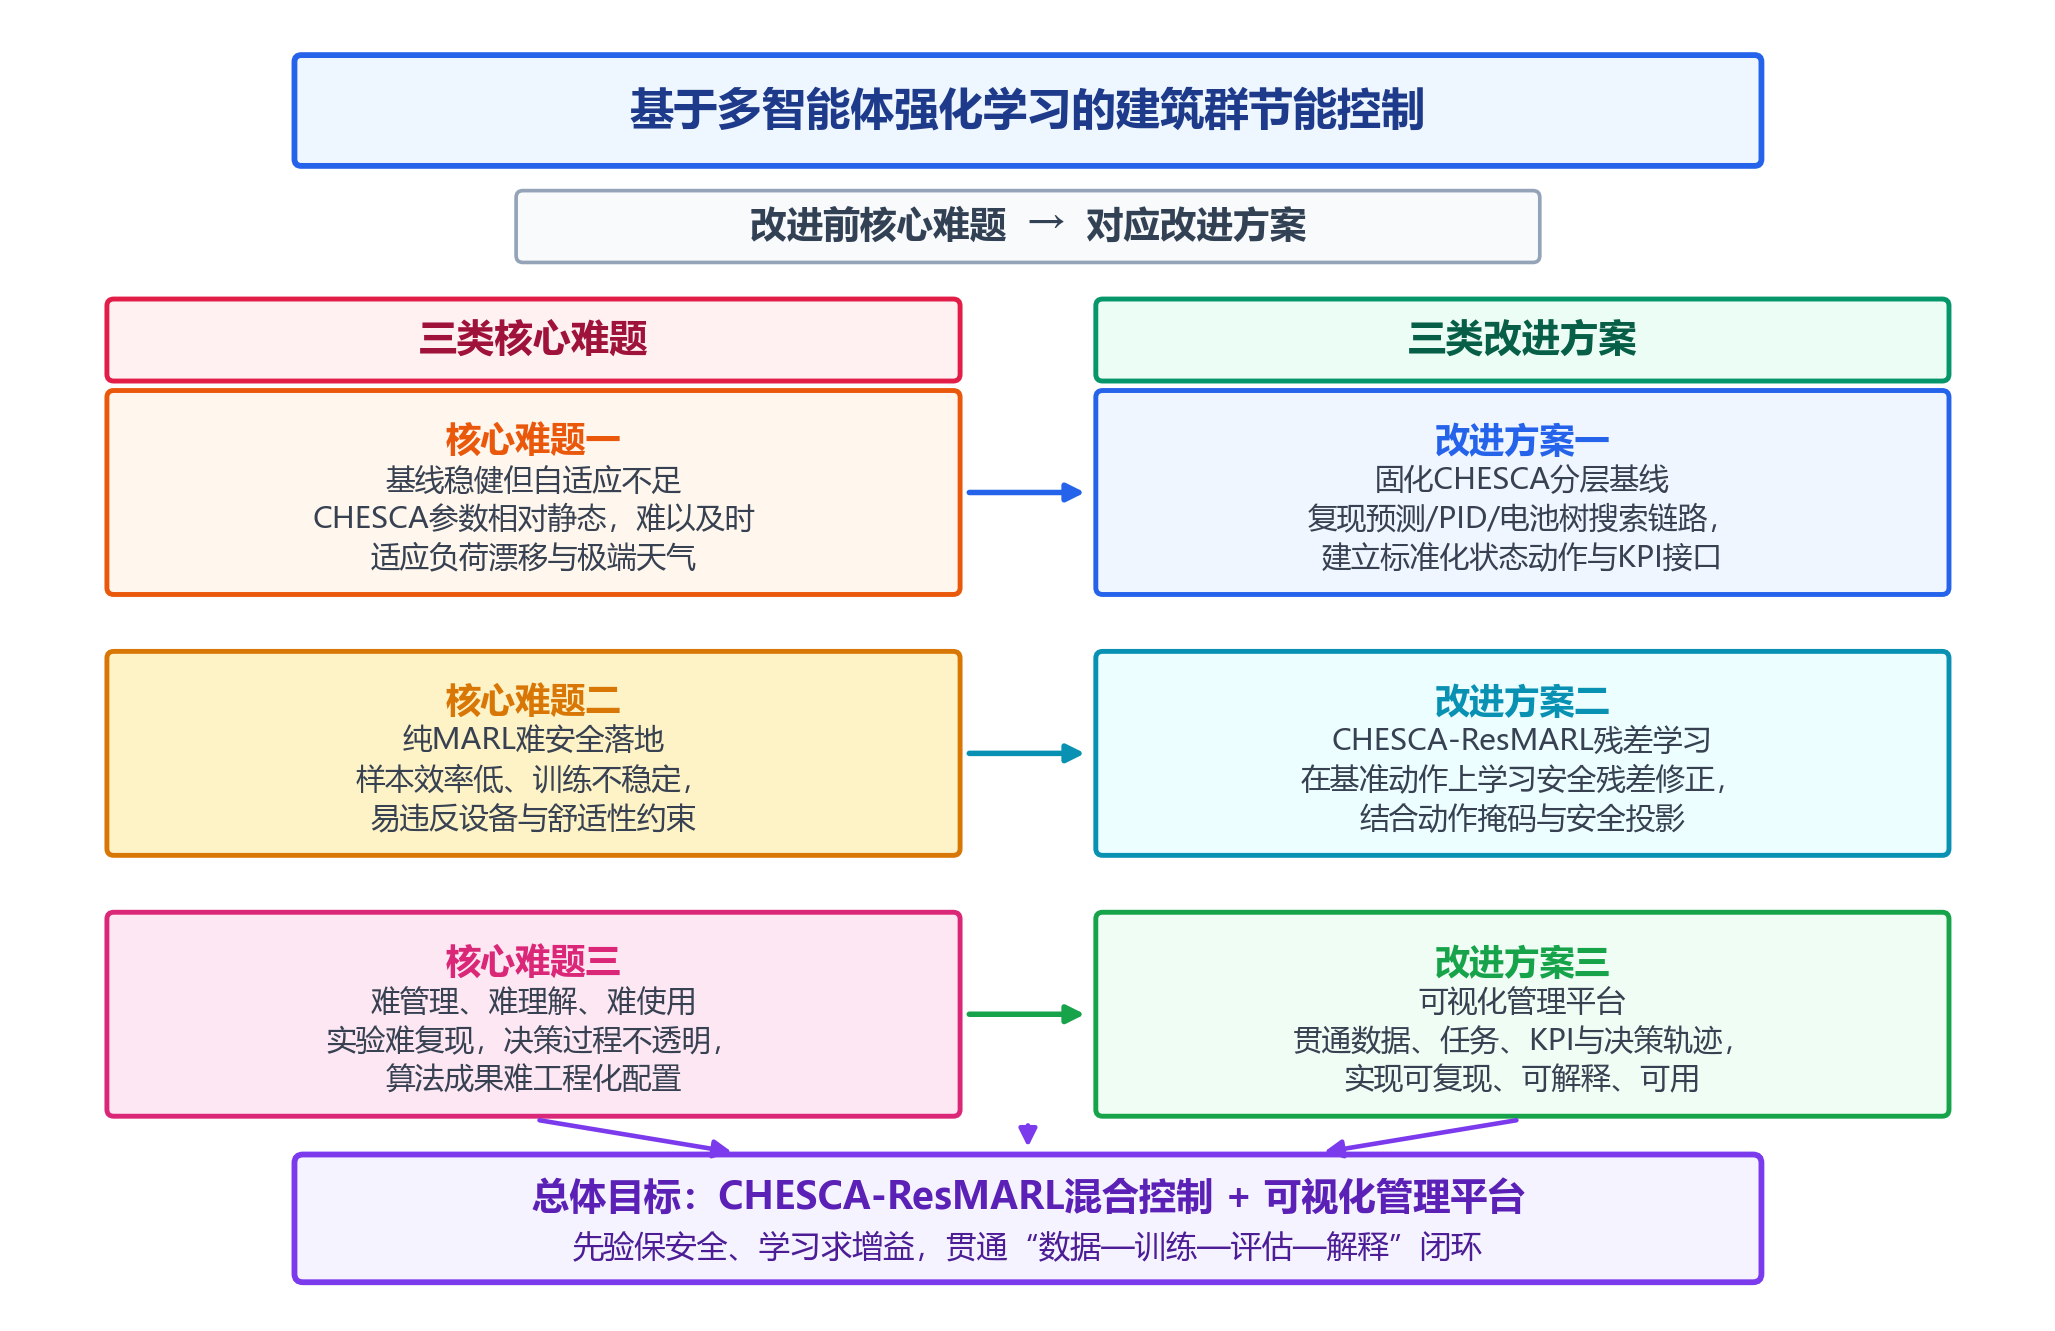
\includegraphics[width=0.92\textwidth]{./images/pictures/核心难题与改进方案.png}
    \centering\bicaption{核心难题与改进方案}{Core Challenges and Improvement Solutions}
    \label{核心难题与改进方案}
\end{figure}

\section{改进前的核心难题与改进方案}
\subsection{改进前的核心难题}
从竞赛算法到可复现、可解释、可部署的系统，本文识别出三类不可回避的核心难题。

（1）难题一：基线稳健但自适应能力不足。CHESCA依靠预测、规则与电池搜索给出了可解释的控制基准，在数据有限的条件下亦能稳定运行。然而其PID增益、搜索权重与电价分位阈值相对固定，面对负荷漂移、设备老化、电价机制调整与极端天气时响应迟缓；当电价机制、设备特性与舒适度要求发生变化时，固定策略只能维持基本可用水平，无法充分挖掘安全边界内的潜在增益。

（2）难题二：纯学习方法性能潜力大但难以安全落地。将建筑建模为智能体后，长期协同策略确实可以通过学习获得，但在CityLearn这类连续动作、强耦合场景中，样本效率低、环境非平稳、信用分配困难与探索不安全等问题同时存在。随机探索可能越过SOC、功率或舒适度边界；在预算有限且缺乏安全层的条件下，纯MARL很难一次性达到工程可接受的稳定性与可复现性。

（3）难题三：实验管理分散、决策过程不透明、成果难以复用。单次实验同时产生配置快照、时序观测、动作轨迹与多维KPI。缺乏统一的数据管理、任务调度与归档机制时，实验复现无从谈起；仅提供最终KPI而不展示基线动作、残差修正与投影过程，运维人员无法理解``为何如此调节''；算法分散于各类脚本之中，非算法背景人员难以完成配置、比较与应用。

\subsection{对应的改进方案}
本文以CityLearn为仿真基准、CHESCA为工程基线，提出CHESCA-ResMARL混合控制策略并构建配套可视化平台。总体思路可以概括为：CHESCA保障动作的可行性与安全性，残差MARL在受限范围内进行策略修正，平台实现实验管理与决策解释的全程贯通。

（1）方案一：复现并固化CHESCA，建立标准化实验链路。梳理预测层、本地动作初稿、未来用电估计、社区电池树搜索与净负荷回写各环节；统一建筑与社区的状态、动作、约束与KPI接口，使NOCONTROL、纯CHESCA与混合策略能够在相同数据与指标体系下进行比较。该方案回应难题一，同时为残差学习提供可退化的安全锚点。

（2）方案二：CHESCA-ResMARL残差多智能体框架。在基准动作$a^{base}$基础上，各建筑智能体依据本地观测输出连续残差，以
\begin{equation}
a^{final}=\mathrm{clip}\big((1-\alpha)a^{base}+\alpha a^{RL}\big)
\end{equation}
或等价的$a^{base}+\alpha\Delta a$形式合成最终动作。利用残差系数$\alpha$、通道掩码（DHW/ELE/TMP）与安全投影将探索范围约束在边界之内；强化学习侧为每栋建筑独立的SAC策略，执行阶段仅依赖本地观测。该方案回应难题二，实现``先验保安全、学习求增益''的设计目标。

（3）方案三：算法—平台一体化的可视化管理。基于Vue、Spring Boot、MySQL与Python算法组件，覆盖权限管理、数据集管理、算法登记、参数配置、异步仿真、KPI图表、决策轨迹与日志归档等功能。以任务标识贯通配置、运行与结果数据，使研究者能够复现实验，管理者能够理解基线、残差与投影如何合成最终动作。该方案回应难题三。

本文的具体研究内容包括：问题建模、CHESCA复现、残差策略与多目标奖励设计及评价、平台研发。潜在贡献为：面向CityLearn场景的CHESCA-ResMARL分层残差框架；兼容规则规划、强化学习、任务调度与KPI分析的一体化接口；在可运行系统中贯通``数据—训练—评估—解释''完整链路。

\section{论文组织结构}
全文共分六章。第一章为引言，阐述建筑群节能控制的现实需求与理论难点，综述国内外研究现状，给出难题—方案总体框架；第二章介绍相关工作与技术，涵盖强化学习、平台技术、残差控制与CityLearn，并单设一节详细解析CHESCA三类动作生成技术与XGBoost预测方法；第三章进行系统需求与架构分析；第四章阐述系统构建与技术实现，单列前端系统功能介绍并预留界面截图位置；第五章给出实验与结果分析，包括Postman接口测试、日志分析与结果可视化；第六章为讨论与展望。

\chapter{相关工作与技术}

\section{强化学习基础}
强化学习是一种通过智能体与环境的交互来学习最优行为策略的机器学习方法\cite{citylearn2020}。智能体、动作、环境、状态和奖励在强化学习中相互关联、相互作用，共同构成了一个完整的学习系统。建筑群能源控制可以抽象为马尔可夫决策过程$(S,A,P,R,\gamma)$：状态$s_t\in S$包含气象、电价、负荷和设备信息，动作$a_t\in A$为设备设定值，转移$P(s_{t+1}|s_t,a_t)$由建筑热动态与设备物理决定，奖励$r_t$反映成本与舒适性。强化学习目标是寻找策略$\pi(a|s)$最大化期望折扣回报，如式\ref{eq:rl-obj}所示。
\begin{equation}
\label{eq:rl-obj}
J(\pi)=\mathbb{E}_{\pi}\left[\sum_{t=0}^{T}\gamma^t r(s_t,a_t)\right].
\end{equation}

（1）智能体：在建筑群场景中，每栋建筑或每类设备被建模为独立智能体。智能体观察周遭环境的状态变化，选择并执行相应动作，并根据环境反馈的奖励或惩罚调整决策策略，追求长期累积奖励最大化\cite{marl2021}。

（2）动作：在本文中动作为CityLearn设备设定值向量，对应HVAC温度设定、DHW功率与电池充放电设定。动作的选择是智能体策略的具体体现，不同策略导致不同的负荷曲线与社区峰值。

（3）环境：环境是智能体所处的建筑群物理世界，接受动作输入并产生新的状态与奖励反馈。CityLearn通过Gymnasium接口提供标准化的气象、电价、碳强度与负荷时序，成为多智能体需求响应的公共仿真场所\cite{citylearn2020}。

（4）状态：状态是环境在某一时刻的完整描述。在本文中建筑观测包括室外温度、太阳辐照、电价、碳强度、建筑电/热负荷、室内温度与电池SOC；社区汇总特征包括总负荷、平均SOC与峰值指示。状态可以是离散的，也可以是连续的传感器与时序数据。

\subsection{基于值函数的强化学习算法}
强化学习算法在策略更新和学习方法上可明确划分为两大类：基于值函数的强化学习算法和基于直接策略搜索的强化学习算法。基于值函数的方法核心是学习状态值函数或动作值函数，不断迭代更新直到收敛，再通过贪婪策略选择使值函数最大的动作。在建筑群控制中，DQN用神经网络近似$Q$函数并用经验回放稳定训练\cite{mnih2015}；DDPG针对连续动作引入确定性策略与评论家网络\cite{ddpg2016}。但值函数方法在多建筑连续设定值空间中容易面临维度灾难，需要结合策略搜索或残差结构降低探索复杂度。

\subsection{基于直接策略搜索的强化学习算法}
基于直接策略搜索的方法直接学习从状态到动作分布的映射，通过策略梯度或信赖域方法更新参数。PPO通过裁剪目标限制策略更新步长，提高了训练稳定性\cite{ppo2017}，是本文独立多智能体基线与残差策略训练的参考方法。直接策略搜索天然适合电池充放电、HVAC温度设定等连续动作，但纯策略探索可能产生违反设备约束或舒适性要求的动作，因此本文将其与CHESCA基线结合，仅学习小范围残差修正。

\subsection{多智能体扩展与经验池}
当每栋建筑视为智能体$i\in\{1,\dots,N\}$时，问题变为马尔可夫博弈，联合观测为$\mathbf{o}=(o_1,\dots,o_N)$，联合动作为$\mathbf{a}=(a_1,\dots,a_N)$。主要难点包括环境非平稳性、信用分配与通信约束\cite{marl2021}。集中训练分散执行（CTDE）是主流范式\cite{lowe2017}：训练阶段评论家可访问全局信息，执行阶段策略仅依赖本地观测。MADDPG为每个智能体维护Actor与集中式Critic\cite{lowe2017}；Wilk等进一步提出仅共享离散化``策略意图''而非全部观测的LSD-MADDPG，在保护隐私的同时保持协同\cite{wilk2024}。经验池通过存储历史交互样本并随机采样，打破时序相关性，是稳定多智能体训练的重要机制；本文训练入口据此保存观测、基线动作、残差与KPI增量，供离线复训与消融分析。

\section{可视化技术}
可视化技术作为一种直观高效的信息传递手段，在建筑群能源实验的管理和优化中发挥着不可替代的作用。通过将复杂的负荷时序、KPI权衡与决策过程以图形形式呈现，可视化帮助研究人员快速把握整体性能与局部细节，发现潜在问题与优化方向。
\subsection{Vue}
前端采用Vue与Element UI构建单页应用。Vue的组件化机制将系统首页、模型配置、能源分析与决策轨迹封装为独立组件，通过路由与状态管理组织页面跳转与任务轮询；Element UI提供表单、表格、对话框等基础控件，保证配置页面与任务列表的交互一致性。平台首页聚合社区KPI卡片，模型优选页支持多算法多指标对比，更多信息与决策对话框支持逐步查看基线动作、残差值与掩码记录。

\subsection{Echarts}
图表层采用Apache ECharts库构建，确保数据可视化既美观又高效。页面中心根据展示内容划分为多个独立而相互关联的区域：折线图直观呈现负荷、电价、SOC与室温随时间步变化的趋势；柱状图对比不同算法的KPI；雷达图揭示成本、碳排、峰值、爬坡与舒适性之间的权衡；决策轨迹图同步展示基线动作、残差与投影结果。能源语义色在全平台保持一致：电网使用蓝色、光伏使用橙色、电池使用青绿色。

\section{多智能体强化学习与残差控制}
\subsection{残差强化学习}
残差强化学习将最终动作分解为基线与修正\cite{residual2019}，如式\ref{eq:residual}所示：
\begin{equation}
\label{eq:residual}
a_t = a^{base}_t + \alpha \cdot \Delta a^{RL}_t,\quad \Delta a^{RL}_t\sim\pi_\theta(\cdot|o_t),
\end{equation}
其中$\alpha$为残差幅度系数。基线$a^{base}_t$由CHESCA、RBC或规划器给出，保证基本可行性；策略仅需学习小范围修正，从而降低探索空间与约束违反概率。在机器人控制中该方法显著提高了样本效率\cite{residual2019}。在能源领域，残差结构天然对应``规则保安全、学习求增益''：若策略输出为零则退化为基线；安全投影层再将动作裁剪到物理边界内。本文将残差系数$\alpha$、动作掩码与安全后处理作为可配置项，与CityLearn动作接口解耦。

\subsection{CHESCA社区分层协调思想}
2023年CityLearn Challenge的优胜方案CHESCA采用社区分层结构\cite{chesca2024}。其要点可概括为：日前层利用XGBoost预测未来负荷并进行电价感知规划；社区层计算总负荷修正信号并分配各建筑参考；本地层跟踪参考并通过路径搜索优化电池充放电序列，成本函数综合电价、碳与爬坡惩罚。该方法仅用有限历史数据即取得稳定性能，体现了``规则先验+数据驱动''的优势。CHESCA的局限是参数静态，难以适应负荷漂移；本文在其上叠加ResMARL，正是为了保留其稳定性并引入自适应修正能力。

\subsection{CityLearn仿真环境与评价指标}
CityLearn是基于Gymnasium接口的开源建筑群仿真平台，专为分布式能源资源调度设计\cite{citylearn2020}。其核心贡献是统一任务框架：提供历史气象、电价、碳强度与负荷时序，定义HVAC、DHW与电池动作接口，并给出多目标KPI\cite{citylearn2024}。2020年后每年举办的CityLearn Challenge进一步推动算法在同一数据与指标下比较\cite{citylearnchallenge2023}。CityLearn v2扩展了韧性、住户中心与碳感知能力，支持电网交互式社区管理\cite{citylearn2024}。本文采用的KPI包括用电成本、碳排放、不舒适度、峰值、爬坡、可再生消纳与电网净负荷等。评价时通常以无控制（NOCONTROL）为分母做归一化，以便跨场景比较。BOPTEST等基于Modelica的框架虽物理精度更高，但部署复杂，更适合单体建筑控制器测试\cite{boptest2021}；CityLearn更适合社区级策略快速迭代，因而被本文选为基准。

\section{平台技术与数据管理}
后端采用Spring Boot提供RESTful接口，MySQL持久化用户、社区、建筑、算法任务与KPI，Redis承担任务队列与状态缓存；Python算法组件独立进程运行，通过文件与任务目录与Java交换配置和结果；前后端分离架构使长时间仿真任务可异步执行，前端轮询任务状态并展示中间日志。数据层面，数据库以建筑时序表、环境时序表、算法脚本表、任务表、KPI结果表、算法配置表与数据集目录表组织CityLearn输入、任务状态与评价结果，详细表设计见第三章概念设计与第四章4.3节。

\section{本章小结}
本章介绍了为了深入研究建筑群节能控制与多智能体残差策略，所应具备的理论知识。通过对研究对象——强化学习基础、值函数与策略搜索方法、多智能体扩展的了解，对可视化技术Vue与ECharts的进一步探索，以及对残差控制、CHESCA分层思想、CityLearn环境与平台数据管理的全面总结，为本文后续系统设计、算法实现与可视化管理奠定了理论基础和技术导向。

\chapter{系统需求与架构分析}
\section{需求分析}
前两章已分别阐述三类核心难题与CHESCA三路动作生成技术：基线稳健但自适应不足、纯学习方法性能潜力大但难以安全落地、实验管理分散且决策过程不透明。本章的任务是将上述问题转化为系统需要完成的功能与技术要求。参考同类毕业论文先需求后架构的组织方式\cite{vue2024,xupengtao2020,springboot2024,wangyonghe2016}，本章从三类用户视角切入，依次展开功能需求、非功能需求与架构设计。

首先分析用户角色。能源管理者关注成本节约与削峰效果，偶尔查看决策轨迹；算法研究者需要配置参数、批量执行实验、比较KPI并追踪残差细节；系统管理员负责账号、数据版本与存储运维。已有平台多停留在数据采集展示与阈值报警阶段，缺乏任务调度、版本追踪与决策解释能力，这正是本系统需要弥补的功能缺口。

\subsection{系统功能性需求分析}
系统功能划分为四个部分：系统管理、数据管理、算法与实验管理、可视化分析。

（1）系统管理。包括用户与权限管理、通知与反馈功能。后台支持用户的录入、编辑与查询，并按权限组分配菜单；管理员发布通知后用户端即时推送；问题反馈直达后台，形成``使用—改进''闭环。密码加密存储，上传文件执行白名单校验，接口层过滤SQL注入与XSS攻击。

（2）数据管理。以CityLearn数据集为核心\cite{citylearn2020,citylearn2024,gymnasium2024}，管理社区、建筑、设备与时序数据。支持数据集导入与CSV导出，记录数据集版本、时间范围与建筑数量；数据集目录维护候选数据集及其兼容性标识，任务提交前自动校验动作空间匹配性，不兼容时直接拦截，避免不合规数据进入评估流程。

（3）算法与实验管理。算法库登记可执行脚本（基线控制与残差强化学习两类入口）；任务记录状态与展示名称；配置以键值形式存储残差系数、掩码、安全开关、训练与评估数据集及模型快照。界面支持新增任务、修改参数与删除任务，便于直观比较不同参数配置。日志按任务隔离，标准输出与结构化结果文件一并归档，解析失败时保留原始行并标注原因。

（4）可视化分析。提供三类视图：KPI对比（柱状图与雷达图，呈现成本、碳排放、峰值、爬坡与舒适度的权衡关系）、时序曲线（负荷、电价、SOC、室温）与决策轨迹（基线、残差、掩码、投影的逐步展示）。设计重点不在于视觉效果，而在于使``控制决策的依据''有据可查。

系统功能结构如图\figref{功能模块图}所示。
\begin{figure}[htb]
    \centering
    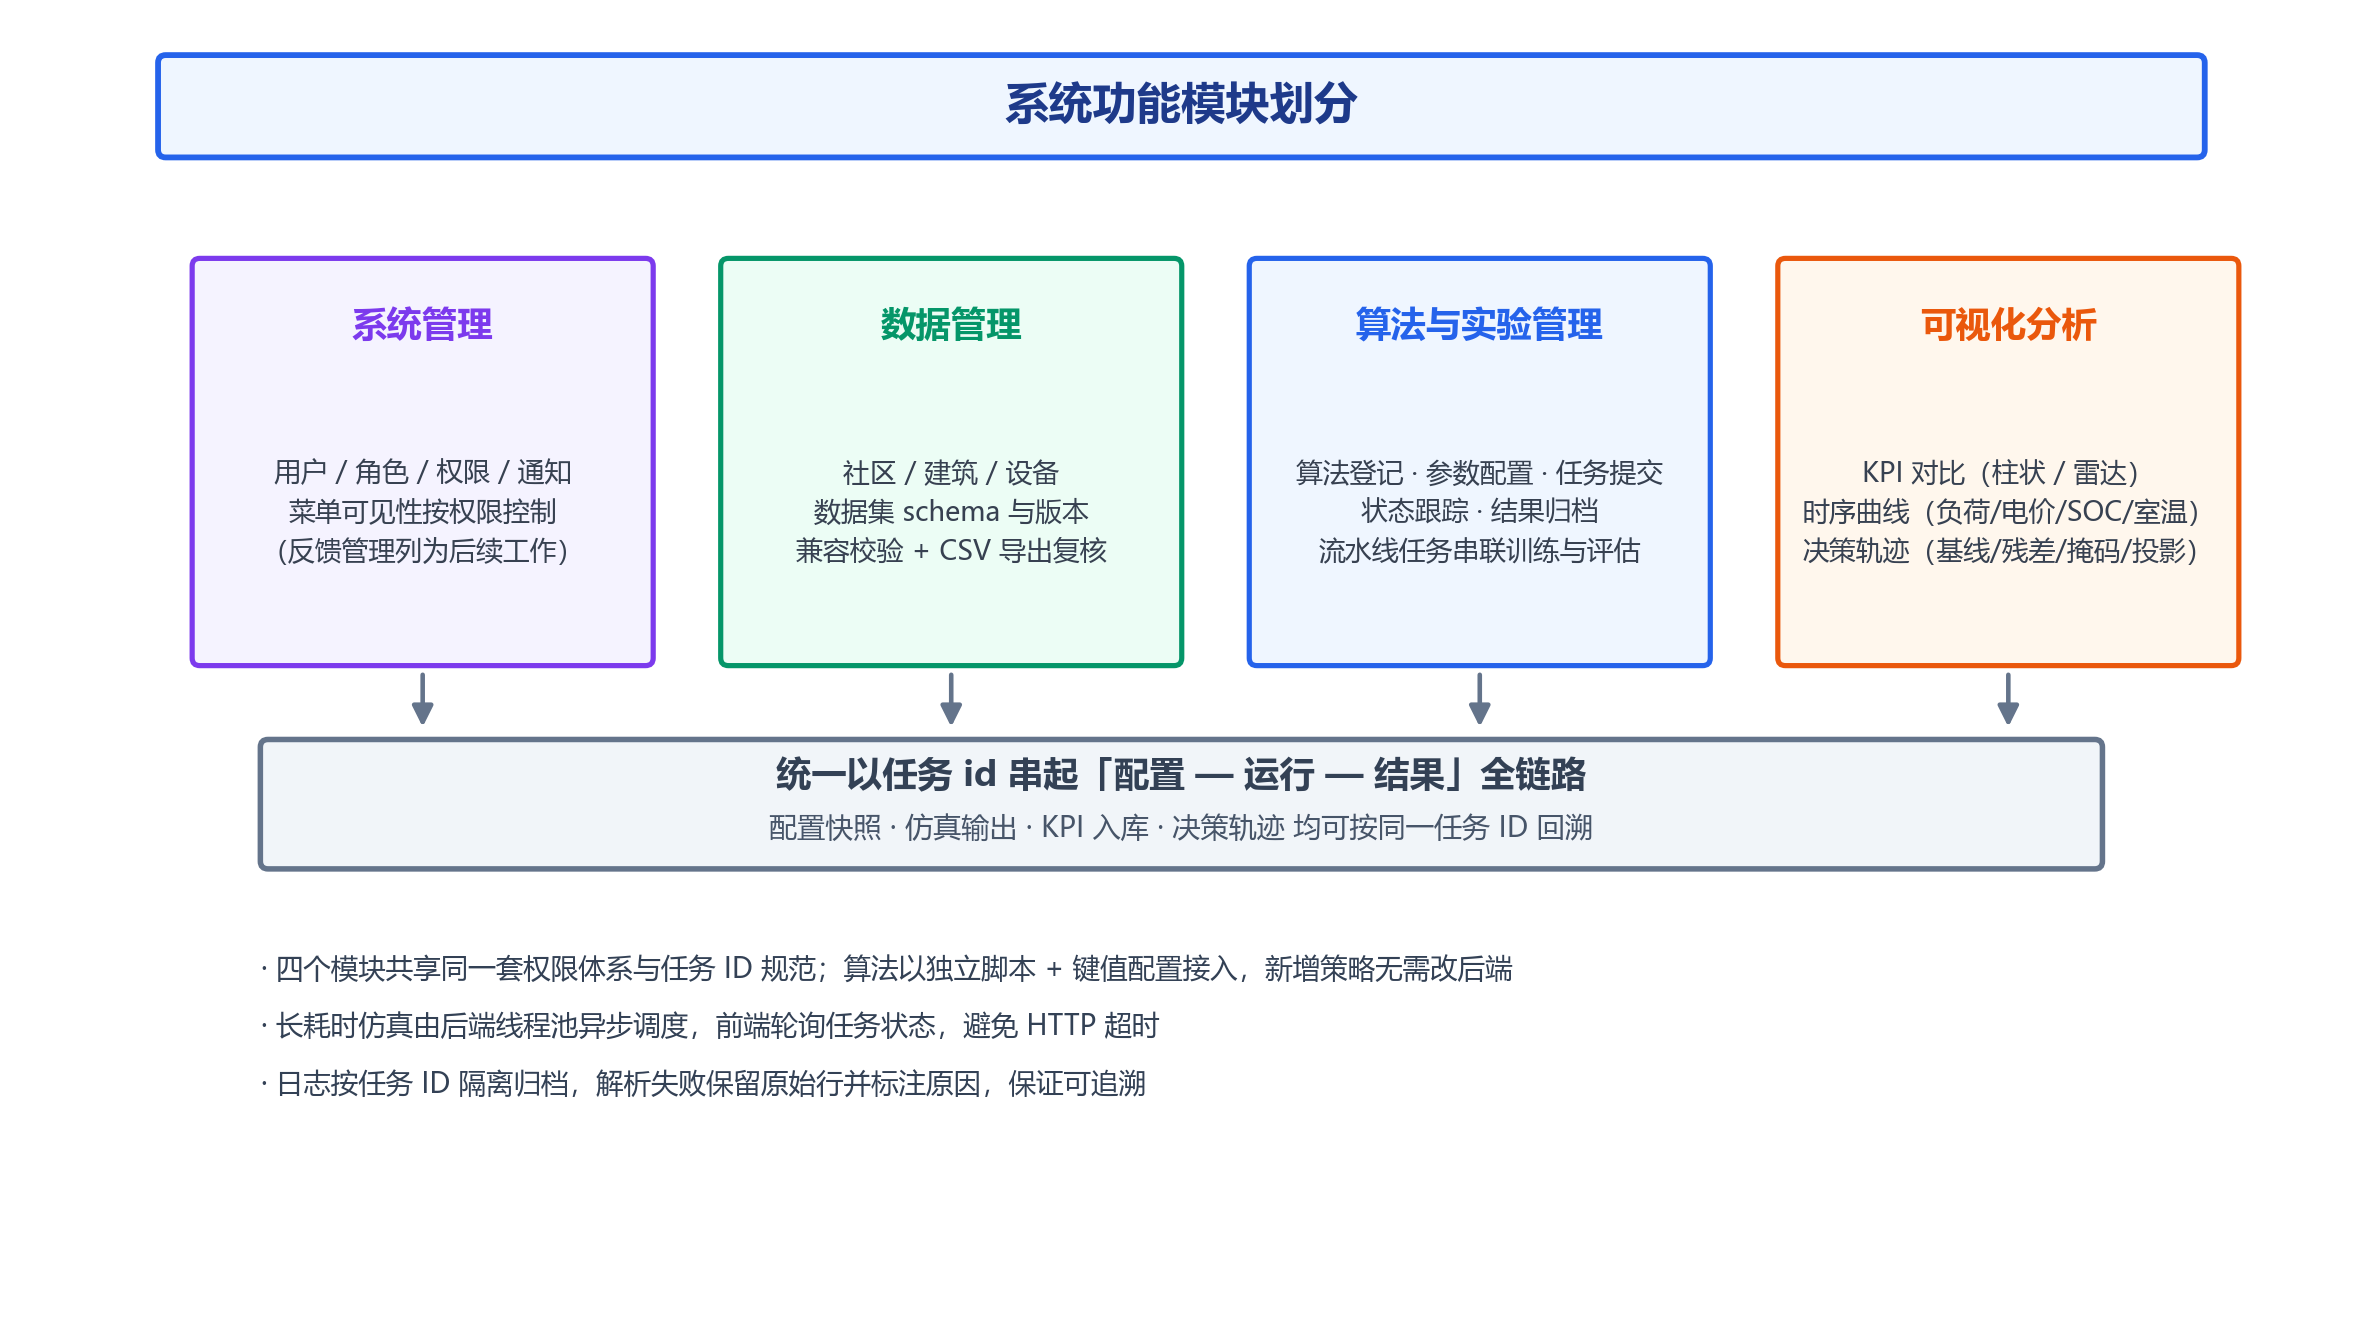
\includegraphics[width=0.92\textwidth]{./images/pictures/功能模块图.png}
    \centering\bicaption{功能模块图}{Functional modules}
    \label{功能模块图}
\end{figure}

\subsection{系统非功能性需求分析}
（1）安全性：权限控制防止越权访问，密码加密存储，上传执行白名单校验，接口过滤注入与脚本攻击，MySQL提供高可靠存储\cite{mysql2024}。

（2）兼容性：系统采用浏览器端渲染，ECharts在Chrome、Edge、Firefox中的表现略有差异\cite{echarts2024}，设计时按最低版本对齐，布局采用Element UI栅格系统\cite{elementui2024}，避免使用私有CSS特性。

（3）可扩展性：算法以独立脚本加键值配置方式接入，新增策略无需修改后端代码；接口遵循RESTful规范\cite{springboot2024}；数据格式标准化并附完整注释，便于后续扩展储能、光伏、电动汽车等设备类型。日志字段先行固化（见4.2节），后续接入ELK/Loki\cite{elk2024}时无需返工。

\section{系统架构设计}
系统采用B/S四层架构：浏览器层、前端Web服务层、后端应用层与数据存储层，如图\figref{系统架构图}所示。
\begin{figure}[htb]
    \centering
    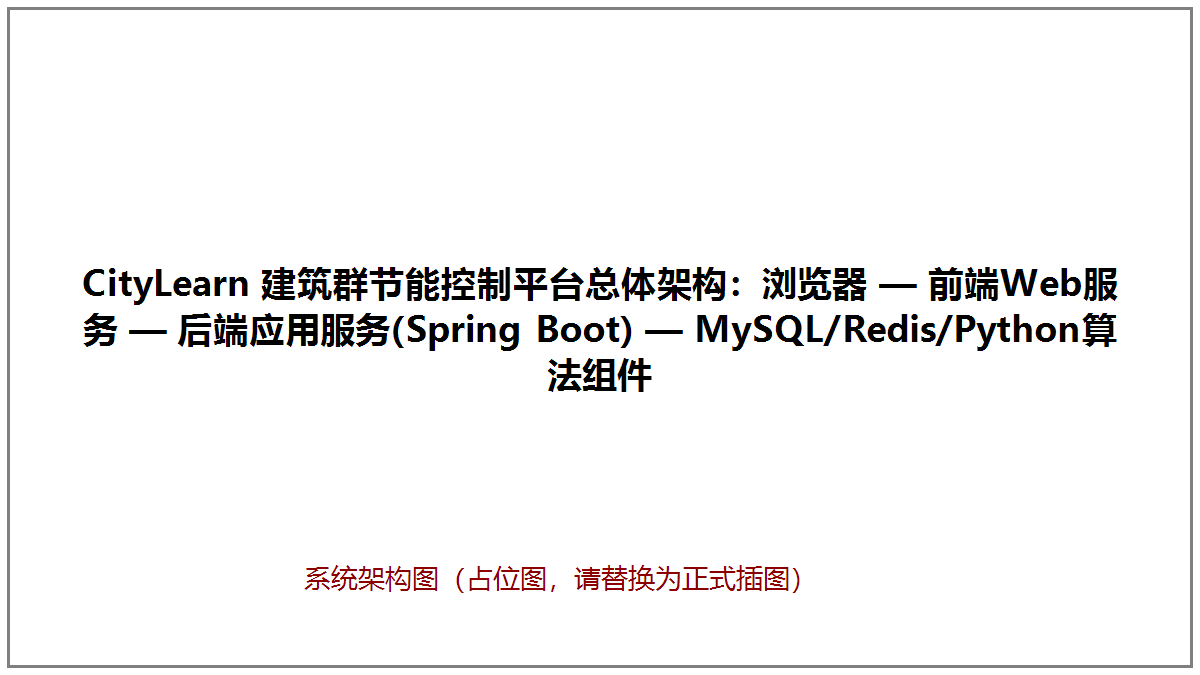
\includegraphics[width=0.85\textwidth]{./images/pictures/系统架构图.png}
    \centering\bicaption{系统架构图}{System Architecture Diagram}
    \label{系统架构图}
\end{figure}

（1）客户端浏览器：负责解析HTML/CSS/JS，渲染页面并执行交互逻辑，管理缓存与隐私数据。

（2）前端Web服务：基于Vue与Element UI构建单页应用\cite{vue2024,xupengtao2020,elementui2024}，采用ECharts绘制KPI与轨迹图表\cite{echarts2024,wangzhiwen2020}。Vue的响应式绑定与组件化机制适用于复杂动态界面开发\cite{xupengtao2020}，Vue、Element UI与ECharts的组合在项目管理平台中已有成熟应用先例\cite{wangzhiwen2020}。该层接收HTTP请求、按路由转发并封装响应，同时承担安全与缓存职能。长耗时任务不阻塞HTTP连接，由前端轮询任务状态。

（3）后端应用服务：基于Spring Boot提供RESTful接口\cite{springboot2024}，负责鉴权、查询、任务提交与状态跟踪，其自动配置与起步依赖机制大幅简化了企业级应用开发\cite{wangyonghe2016}。长耗时仿真任务异步进入队列，遵循``长任务异步、短请求同步''原则，避免请求超时。

（4）数据存储：数据库存储业务数据与指标聚合结果\cite{mysql2024}，基于Java与MySQL的数据库管理系统设计是此类业务系统的常规做法\cite{ouyangguixiu2022}；Python算法组件以独立进程运行CityLearn仿真\cite{citylearn2020,gymnasium2024}，通过HTTP/REST接口接收Java端下发的仿真任务，仿真所需的配置与结果数据经任务目录中的文件交换，实现后端与算法模块的解耦。明细时序数据与结果文件按任务目录落盘，数据库仅保存索引，兼顾查询效率与原始数据可追溯性。

\section{功能模块设计}
\subsection{系统管理模块}
涵盖用户、角色、权限与通知管理。用户管理页面提供用户的录入、编辑、查询与启停维护；角色与权限组控制菜单可见性（如任务列表入口仅对有权限用户可见）；通知以任务完成未读提醒的形式落地，与任务状态联动；问题反馈直达后台，形成``使用—改进''闭环。

\subsection{数据管理模块}
管理社区、建筑、设备与数据集版本。以数据集为单位记录建筑数量、时间步数与兼容性标识，为仿真任务提供统一输入；CSV导出功能支持离线复核。

\subsection{算法与实验管理模块}
覆盖算法登记、参数配置、任务提交、状态跟踪与结果归档。算法参数配置页面以结构化分组表单维护各算法的可配置参数，并支持以在线代码编辑器直接查看与编辑脚本；残差系数、掩码、安全开关与模型文件在提交时进行校验并生成配置快照；任务由后端线程池异步调度执行；任务列表页面支持任务的分页查询、进度轮询、标准输出与错误日志查看；流水线任务支持将多个步骤（如训练与评估）串联为子任务序列。

\subsection{可视化分析模块}
指标对比读取指标汇总数据，支持多任务横向比较与雷达图展示；时序视图按建筑与时间维度绘制负荷、电价、SOC与室温曲线；轨迹视图逐步呈现基线、残差、掩码与投影结果。全系统统一采用任务标识，保证配置、仿真与结果全链路可追溯。核心业务流程为：用户登录后选择数据集与算法，配置参数并提交任务；调度器写入配置并调用Python执行；任务完成后解析指标入库，前端跳转至分析页面。

\section{数据库概念设计}
数据库采用MySQL 8.0 InnoDB引擎，字符集为\texttt{utf8mb4}。数据按业务功能分为三类：第一类为建筑与环境时序数据，承载各建筑的分时观测以及天气、电价、碳强度等外部环境信息；第二类为运行结果数据，承载算法脚本登记、仿真任务状态与各项评价指标；第三类为配置与目录数据，承载算法可调参数与数据集登记信息。

表间联系为：脚本与任务为1:N关系；任务与指标及结果文件为1:N关系；数据集与任务为1:N关系；各类时序数据按时间步号逻辑对齐。如图\figref{数据库E-R图}所示。
\begin{figure}[htb]
    \centering
    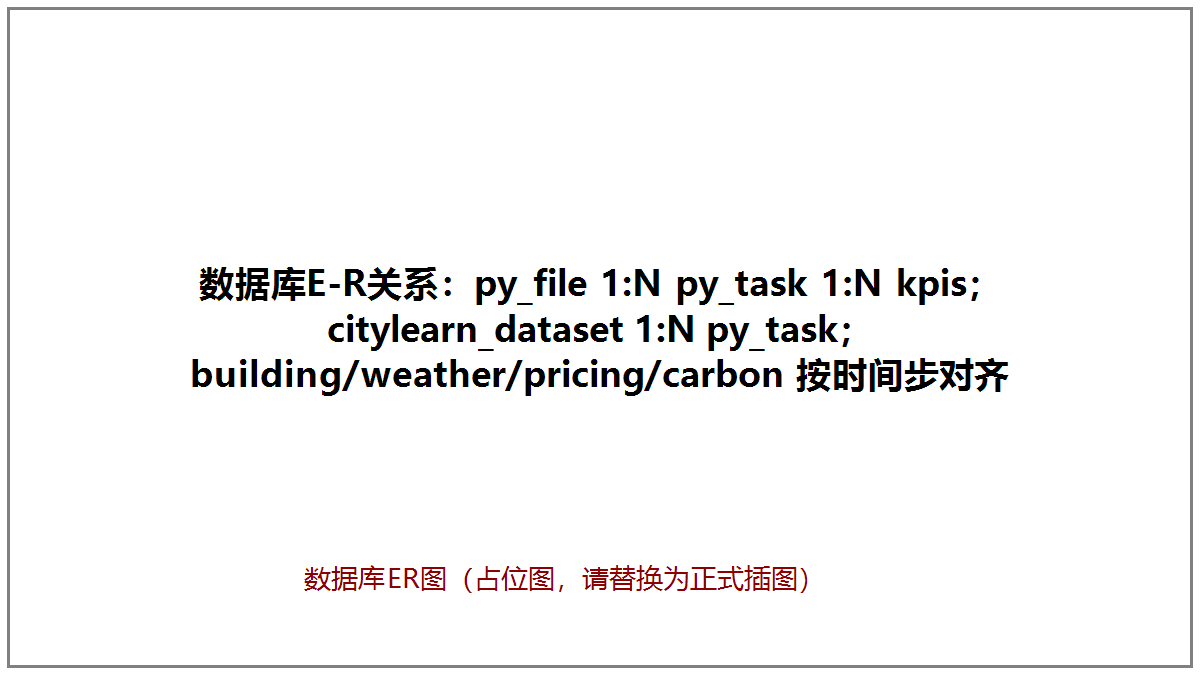
\includegraphics[width=0.85\textwidth]{./images/pictures/数据库ER图.png}
    \centering\bicaption{数据库E-R图}{E-R Diagram of the Database}
    \label{数据库E-R图}
\end{figure}

\section{本章小结}
本章将需求分析转化为架构设计：明确三类用户、四块功能、B/S四层架构，以任务标识贯通全链路。数据库概念设计先行，字段级实现详见4.3节。接口契约与日志规范是下一章的输入，Postman与日志分析的具体做法与2.4、2.5及5.1节相呼应。

\chapter{系统构建与技术实现}
\section{页面设计总览}
本章阐述系统的具体构建过程。参考同类毕业论文先页面、再日志、再存储的组织顺序，本章首先介绍四个核心页面：系统首页、模型配置、能源分析与决策轨迹。页面统一采用Vue与Element UI实现\cite{vue2024,elementui2024}，图表采用ECharts绘制\cite{echarts2024}。后文4.5节单列前端系统功能介绍并预留截图位置，5.1节将介绍Postman如何保障接口契约\cite{postman2024}。

\subsection{系统首页设计}
用户登录后首先进入系统首页。顶部导航分为系统首页、模型配置、能源分析与决策轨迹四个板块，右上角为用户菜单。页面中部大标题点明建筑群节能控制主题，旁设新建仿真任务快捷按钮，便于新用户快速定位功能入口。首页同时聚合社区KPI卡片，默认加载最近一次完成任务的成本、碳排放与峰值指标，无需跳转页面即可获得整体概览。

\begin{figure}[htb]
    \centering
    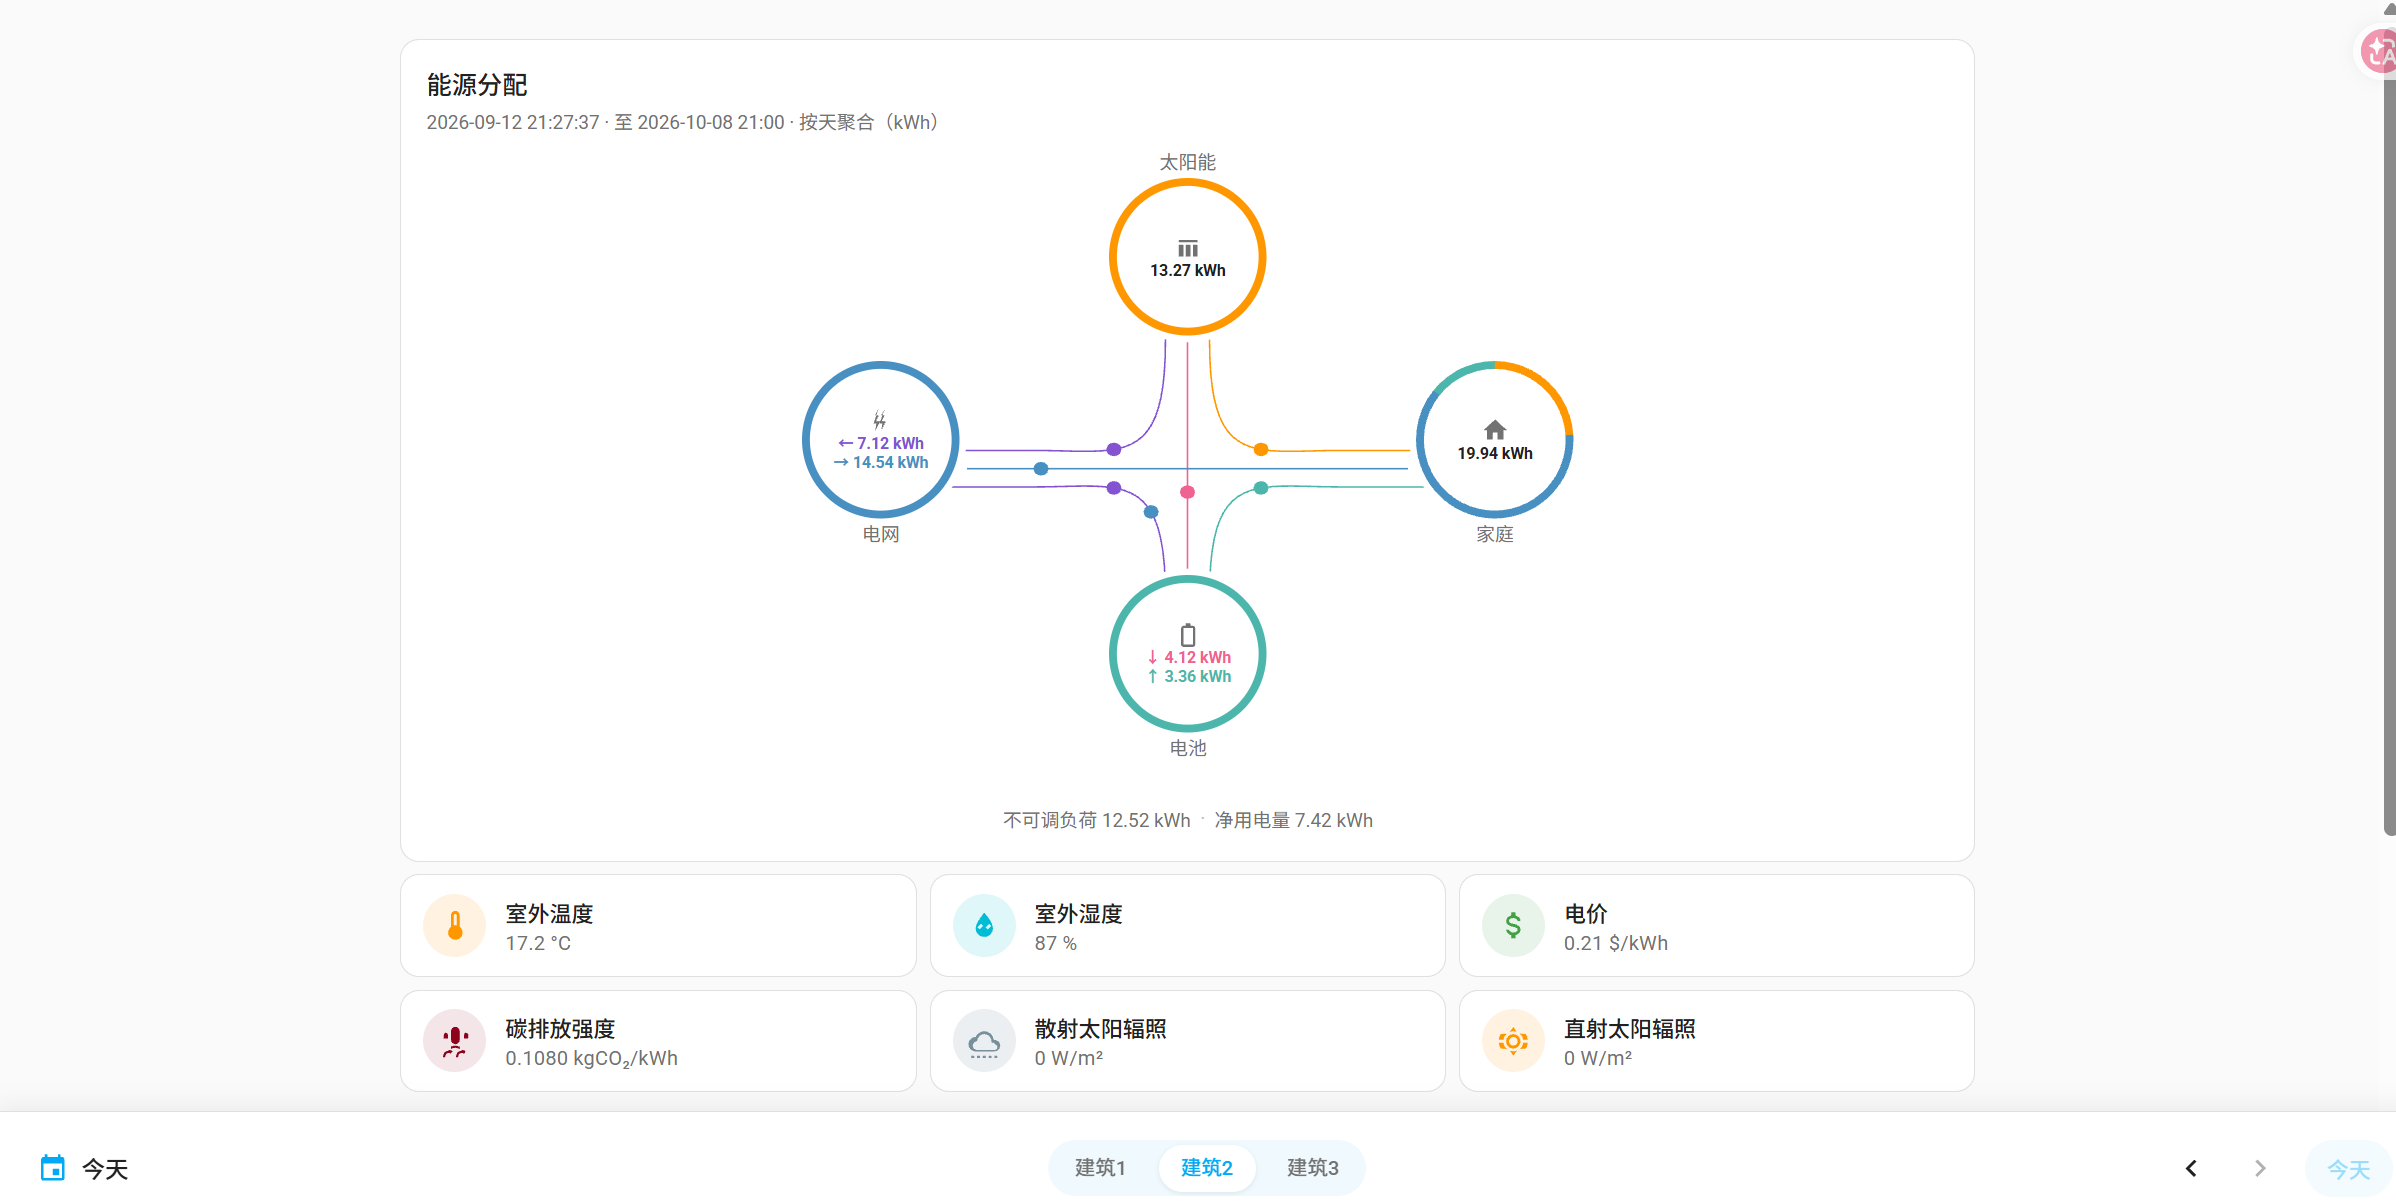
\includegraphics[width=0.85\textwidth]{./images/image/首页.jpg}
    \centering\bicaption{系统首页}{Home page}
    \label{系统首页界面}
\end{figure}

\subsection{算法与数据集配置页面设计}
配置页面的核心是一张带校验规则的表单。字段包括控制器类型、数据集、仿真步数、残差系数、动作掩码、安全投影开关与多智能体模型文件路径。选择纯基线控制时残差相关项自动隐藏；选择残差强化学习模式时模型文件为必填项且需校验数据集兼容性。校验基于表单规则实现\cite{elementui2024}，填写错误时前端直接拦截、不发送请求。提交成功后任务进入列表并实时可见。
\begin{figure}[htb]
    \centering
    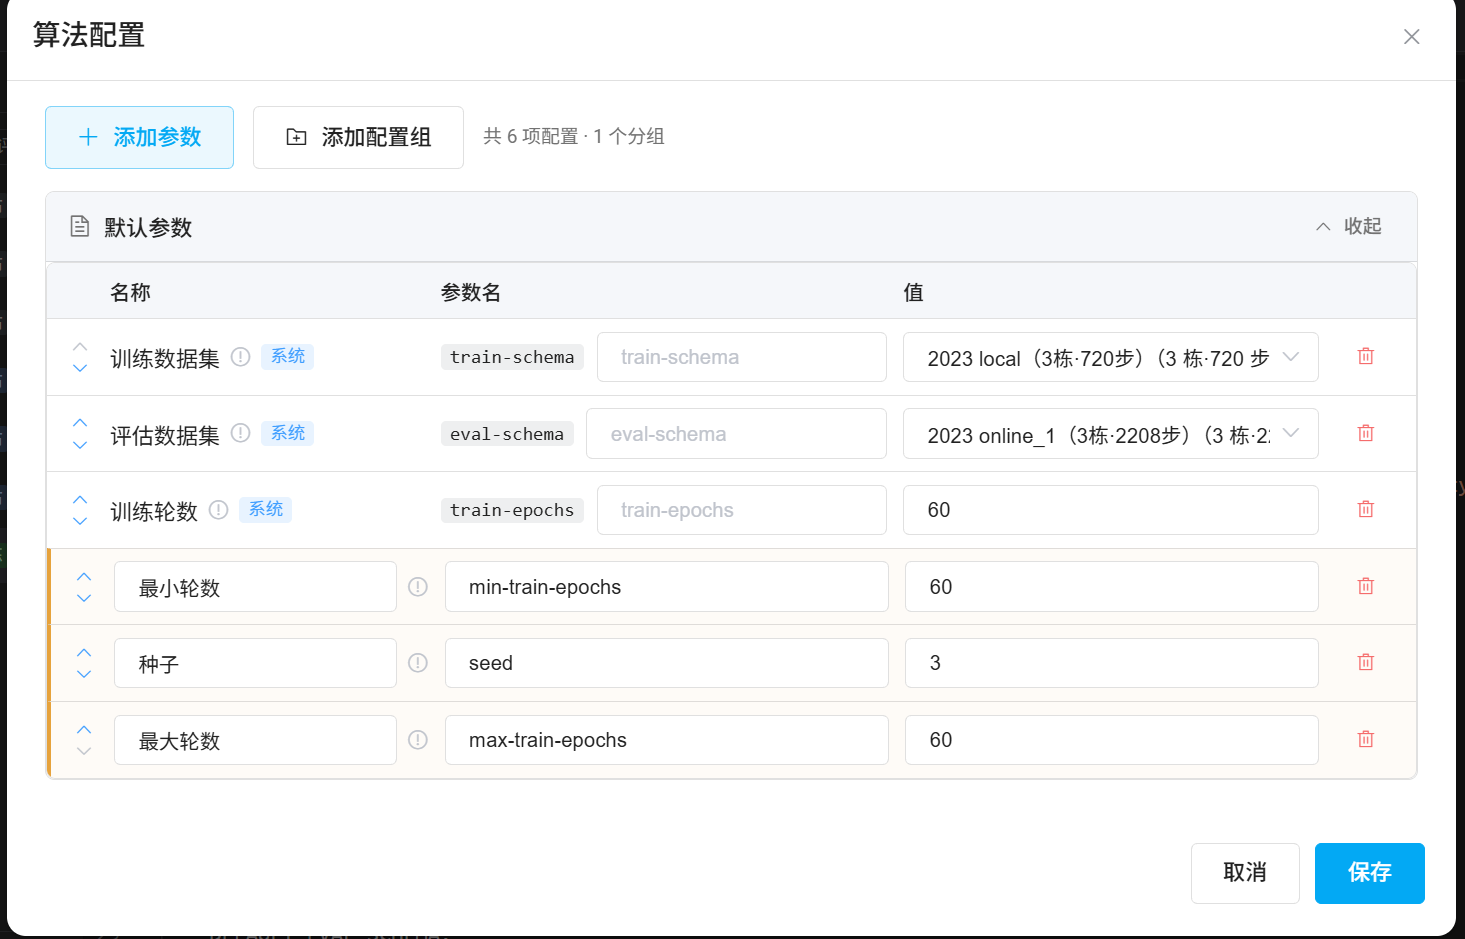
\includegraphics[width=0.85\textwidth]{./images/image/算法配置页.jpg}
    \centering\bicaption{模型配置页}{Model config page}
    \label{模型配置页面}
\end{figure}

\subsection{能源与KPI分析页面设计}
分析页面采用分块多图布局。折线图展示负荷与电价随时间步的变化，柱状图比较不同算法的KPI，雷达图呈现五维指标权衡。首次进入页面自动加载默认任务，检索框支持按任务标识回溯历史任务。全平台配色统一：电网蓝、光伏橙、电池青绿，多任务对比时不会发生混淆。
\begin{figure}[htb]
    \centering
    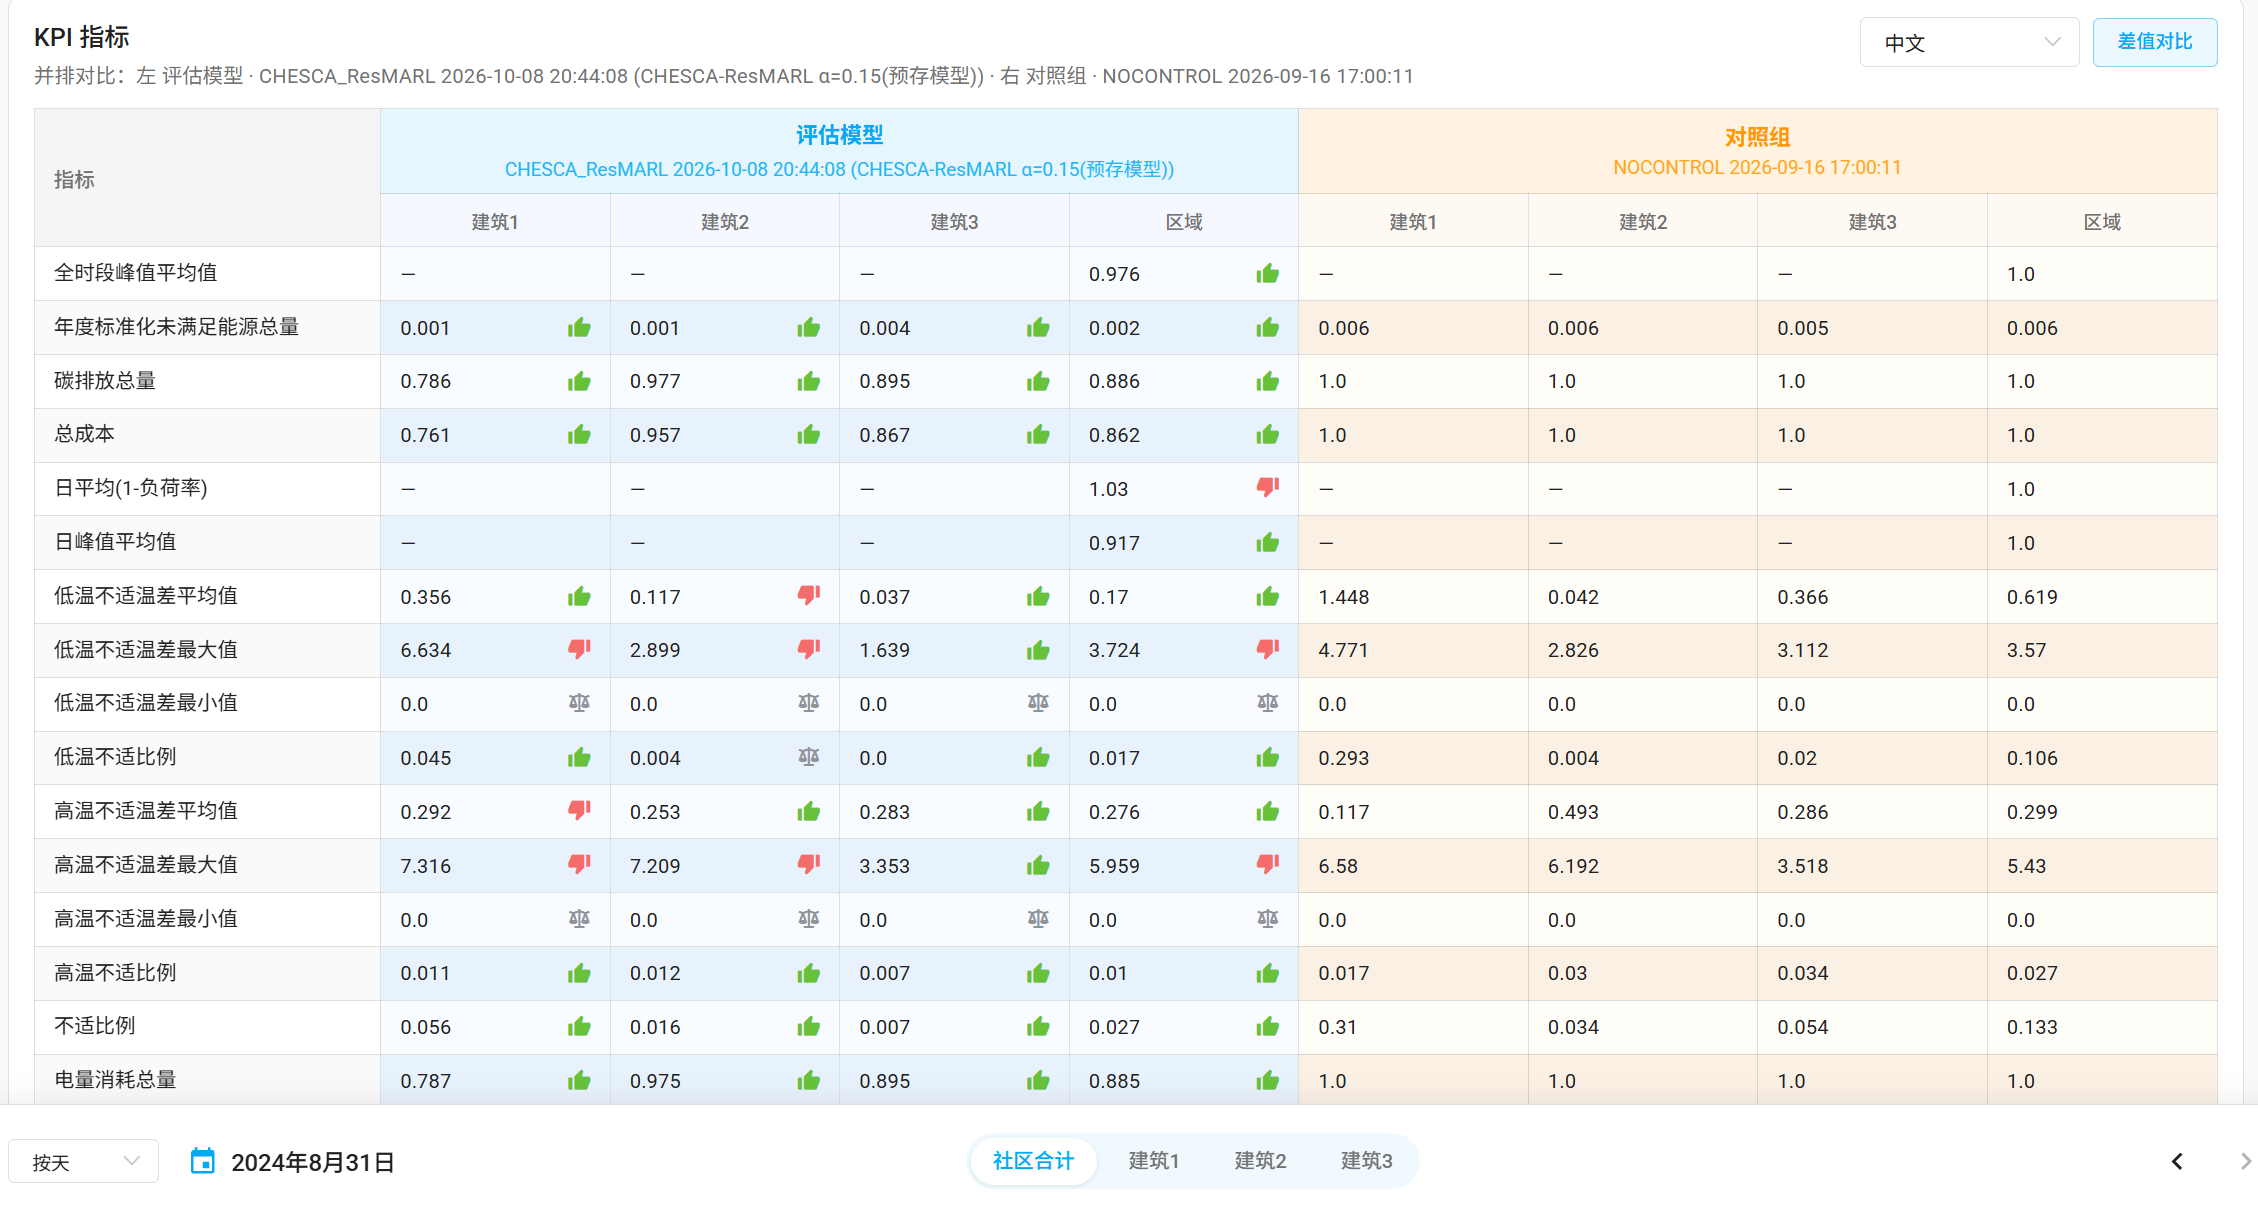
\includegraphics[width=0.85\textwidth]{./images/image/指标对比.jpg}
    \centering\bicaption{能源KPI分析页}{KPI analysis page}
    \label{能源KPI分析页面}
\end{figure}

\subsection{决策轨迹页面设计}
轨迹页面按时间步读取决策推演日志与决策记录，将基线动作、原始残差、掩码、投影后动作、SOC与舒适度状态绘制于同一时间轴。定位至峰值时段后，可直接观察残差是否被安全层约束，较仅查看最终指标更具诊断价值。该页面由轨迹面板、决策记录日志与残差增量展示等一组组件协作实现，分别负责轨迹主视图渲染、逐步决策记录回放与各通道残差增量的可视化。
\begin{figure}[htb]
    \centering
    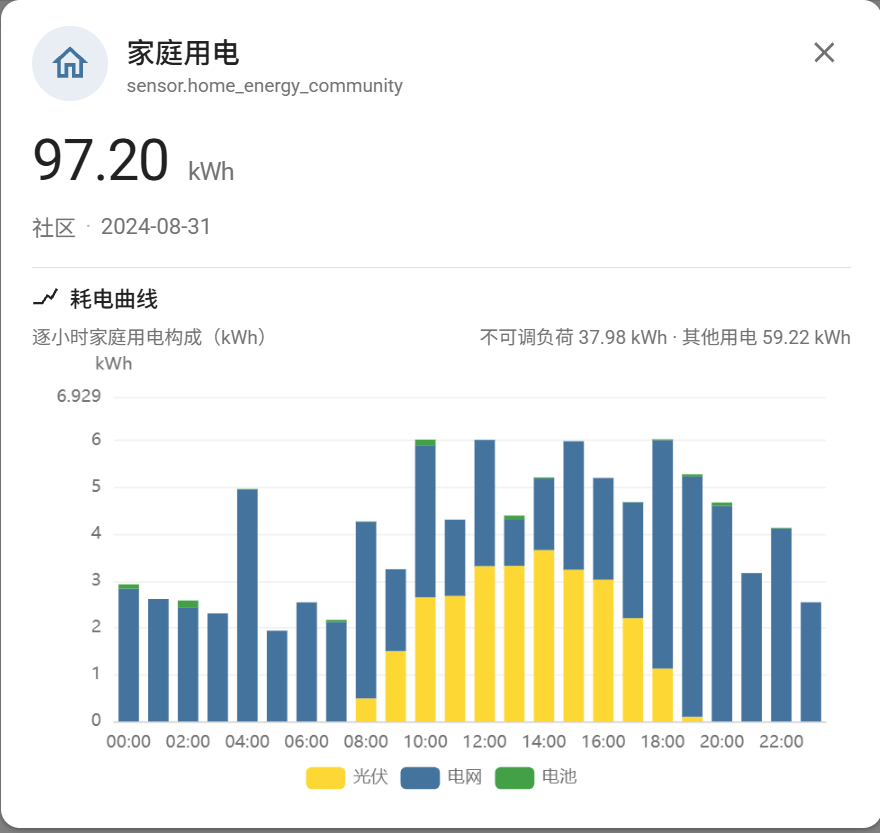
\includegraphics[width=0.85\textwidth]{./images/image/环境状态1.jpg}
    \centering\bicaption{决策轨迹页}{Decision trace page}
    \label{决策轨迹页面}
\end{figure}

\section{日志的自动化与规范化管理}
日志部分需首先交代现状：项目目前尚未部署独立日志平台，采用文件日志、任务目录归档与数据库状态字段相结合的组合方案。Python标准输出重定向至任务目录，配置、指标与轨迹文件按任务标识隔离；Java端读取退出码更新任务状态，解析失败时保留原始行并标注原因。问题排查主要检查三个文件：运行日志、算法指标与决策推演日志。

日志规范分为三个环节。第一，自动化解析：日志中混合配置、奖励与指标等信息，采用正则表达式提取字段，提取失败时记录原始行与原因，不做静默丢弃。第二，规范导出：解析结果按结构化文件格式落盘，字段名与数据库保持一致，时间步从0开始连续编号，缺失步需显式标注。第三，持久化：明细数据经事务写入数据库，指标聚合结果写入指标汇总数据，明细数据保留在文件中，数据库仅保存索引。并发任务采用多线程或异步写入，互不阻塞。

集中式日志方案作为备选，当前阶段不强制部署。待日志规模增长后接入ELK或Loki\cite{elk2024}：采集组件采集各节点日志，按任务标识、控制器类型与数据集类型打标签，Kibana按任务查询全链路日志。字段规范在本节固化，后续仅需增加采集组件，无需返工。日志流水线如图\figref{日志流水线图}所示。
\begin{figure}[htb]
    \centering
    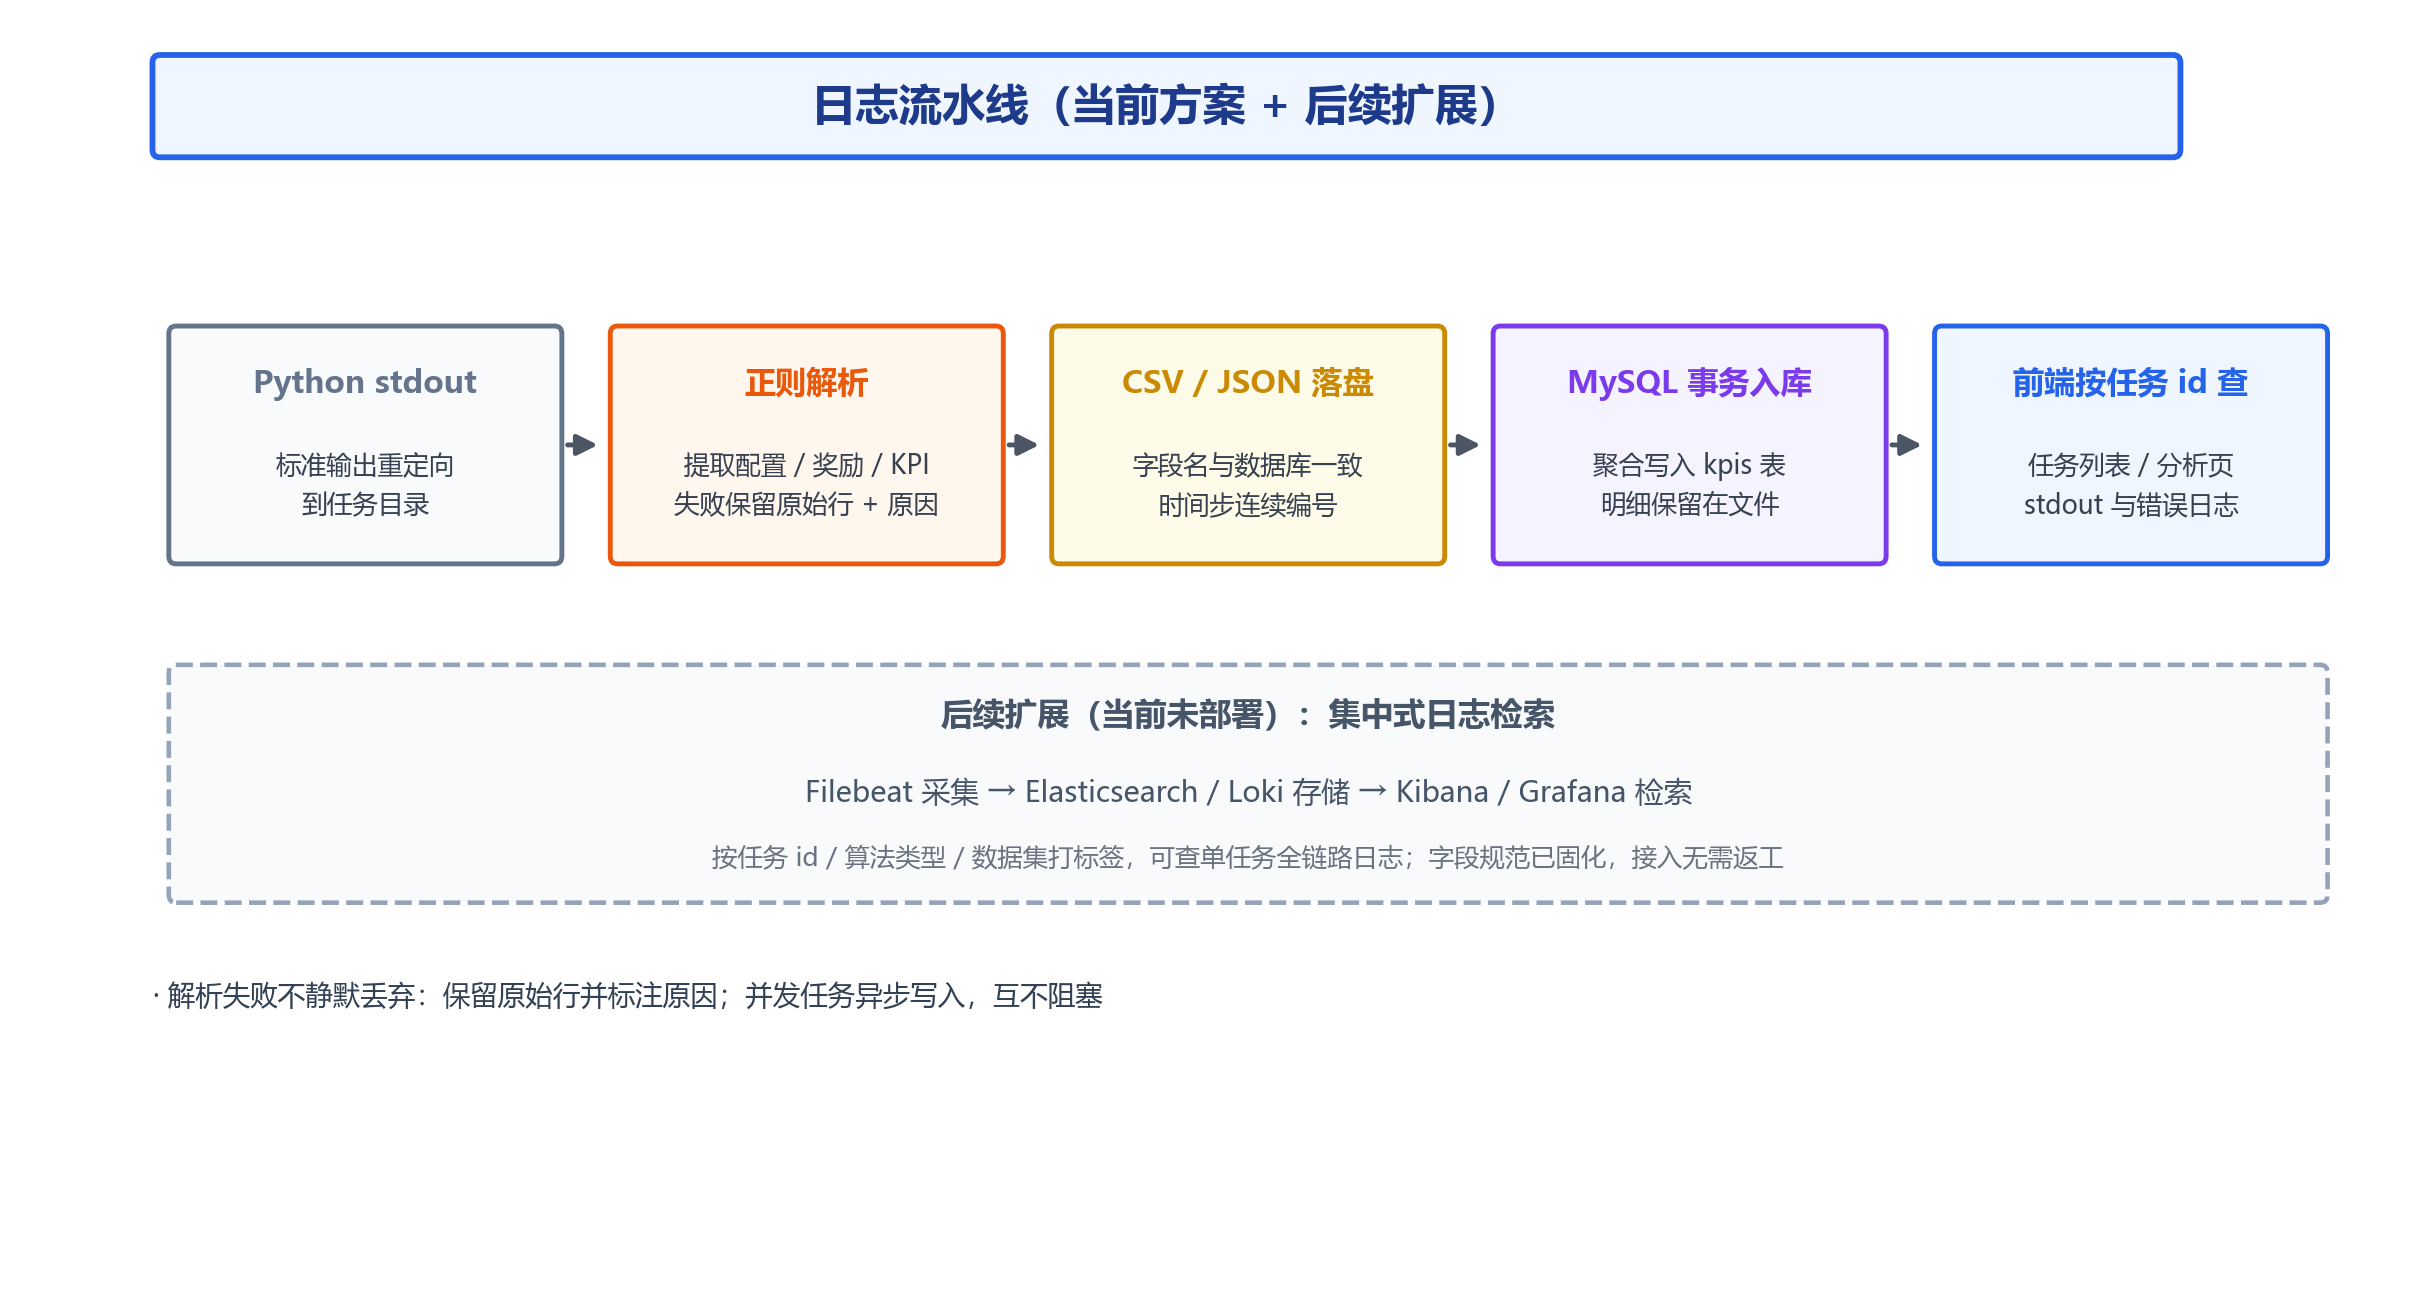
\includegraphics[width=0.92\textwidth]{./images/pictures/日志流水线图.png}
    \centering\bicaption{日志流水线图}{Log pipeline}
    \label{日志流水线图}
\end{figure}

\section{数据库设计与实现}
数据库采用MySQL 8.0 InnoDB引擎，字符集\texttt{utf8mb4}。数据表按业务功能分为五组：建筑时序、环境时序、算法脚本与任务、评价指标、配置与目录。

（1）建筑时序表，如表\ref{tab:building-table}所示。各建筑对应的表结构相同，按建筑区分存储，存储月份、小时、日类型、夏令时、室内温湿度、未满足冷设定点差、不可转移负荷、热水/冷热需求、光伏发电、占用人数、设定点与HVAC模式。主键按时间步连续编号，与CityLearn观测一一对应，前端曲线直接读取。
\begin{table}[h!]
    \centering\bicaption{建筑时序表设计}{Design of building time-series table}
    \label{tab:building-table}
    \begin{tabular}{P{14em}P{6em}P{4em}P{8em}}
        \toprule
        字段名 & 数据类型 & 非空 & 注释 \\\midrule
        id & bigint & 是 & 时间步主键 \\
        month & int & 否 & 月份 \\
        hour & int & 否 & 小时 \\
        day\_type & int & 否 & 日期类型 \\
        daylight\_savings\_status & int & 否 & 夏令时状态 \\
        indoor\_dry\_bulb\_temperature & decimal(14,9) & 否 & 室内干球温度 \\
        average\_unmet\_cooling\_setpoint\_difference & decimal(14,9) & 否 & 未满足冷设定点差 \\
        indoor\_relative\_humidity & decimal(14,9) & 否 & 室内相对湿度 \\
        non\_shiftable\_load & decimal(14,9) & 否 & 不可转移电负荷 \\
        dhw\_demand & decimal(14,9) & 否 & 生活热水需求 \\
        cooling\_demand & decimal(14,9) & 否 & 制冷需求 \\
        heating\_demand & decimal(14,9) & 否 & 制热需求 \\
        solar\_generation & decimal(14,9) & 否 & 太阳能发电量 \\
        occupant\_count & int & 否 & 占用人数 \\
        cooling\_set\_point & decimal(14,9) & 否 & 制冷设定点 \\
        heating\_set\_point & decimal(14,9) & 否 & 制热设定点 \\
        hvac\_mode & int & 否 & HVAC模式 \\
        \bottomrule
    \end{tabular}
\end{table}

（2）环境时序表，如表\ref{tab:env-table}所示。天气表存储室外温湿度、散射与直射辐照度及三步预测值；电价表存储实际电价与预测电价；碳强度表存储排放因子。自增id与建筑表时间步隐式对齐，不建立跨表外键，由应用层校验行数与顺序，防止数据错位。
\begin{table}[h!]
    \centering\bicaption{环境时序表设计}{Design of environment time-series tables}
    \label{tab:env-table}
    \begin{tabular}{P{14em}P{6em}P{4em}P{8em}}
        \toprule
        字段名 & 数据类型 & 非空 & 注释 \\\midrule
        \multicolumn{4}{l}{天气表} \\
        id & bigint & 是 & 时间步主键 \\
        outdoor\_dry\_bulb\_temperature & decimal(12,2) & 否 & 室外干球温度 \\
        outdoor\_relative\_humidity & decimal(12,2) & 否 & 室外相对湿度 \\
        diffuse\_solar\_irradiance & decimal(12,2) & 否 & 散射辐照 \\
        direct\_solar\_irradiance & decimal(12,2) & 否 & 直射辐照 \\
        outdoor\_temperature\_predicted\_1--3 & decimal(12,6) & 否 & 温度预测值 \\
        outdoor\_humidity\_predicted\_1--3 & decimal(12,6) & 否 & 湿度预测值 \\
        solar\_irradiance\_predicted\_1--3 & decimal(12,6) & 否 & 辐照预测值 \\
        \multicolumn{4}{l}{电价表与碳强度表} \\
        id & bigint & 是 & 时间步主键 \\
        electricity\_pricing & decimal & 否 & 实际电价与预测电价 \\
        carbon\_intensity & decimal & 否 & 碳排放因子 \\
        \bottomrule
    \end{tabular}
\end{table}

（3）算法脚本与任务表，如表\ref{tab:py-table}所示。算法脚本表存储脚本名称（基线控制与残差强化学习两类入口）、说明、是否内置及创建审计信息；仿真任务表存储任务标识、关联脚本、状态（0执行中、1完成、2失败）、逻辑删除标记、是否展示与展示名称。结果文件按任务目录落盘，数据库仅保存索引。
\begin{table}[h!]
    \centering\bicaption{算法脚本与仿真任务表设计}{Design of algorithm script and task tables}
    \label{tab:py-table}
    \begin{tabular}{P{10em}P{8em}P{4em}P{10em}}
        \toprule
        字段名 & 数据类型 & 非空 & 注释 \\\midrule
        \multicolumn{4}{l}{算法脚本表} \\
        id & varchar(64) & 是 & 脚本标识 \\
        file\_name & varchar(255) & 否 & 脚本文件名 \\
        desc & varchar(500) & 否 & 算法说明 \\
        if\_system & tinyint(1) & 否 & 是否系统脚本 \\
        create\_time & datetime & 否 & 创建时间 \\
        create\_user & varchar(64) & 否 & 创建人 \\
        \multicolumn{4}{l}{仿真任务表} \\
        id & varchar(64) & 是 & 任务标识 \\
        py\_id & varchar(64) & 否 & 关联脚本标识 \\
        status & int & 否 & 执行状态 \\
        if\_delete & tinyint(1) & 否 & 逻辑删除标记 \\
        if\_show & tinyint(1) & 否 & 是否展示 \\
        show\_name & varchar(128) & 否 & 仪表盘展示名称 \\
        create\_time & datetime & 否 & 创建时间 \\
        update\_time & datetime & 否 & 更新时间 \\
        \bottomrule
    \end{tabular}
\end{table}

（4）评价指标表，如表\ref{tab:kpi-table}所示。存储任务或算法名称、控制器类型及一系列归一化指标字段：全时段峰值、未满足能源、碳排放、成本、日月负荷率、日峰值、冷热不适、总用电量、热韧性、停电未满足、爬坡与零净能耗。前端表格、柱状图与雷达图直接读取本表；逐时明细数据走文件通道。该表以任务名称与控制器类型作为检索依据，配合任务标识保证结果唯一归属。
\begin{table}[h!]
    \centering\bicaption{KPI结果表设计}{Design of KPI result table}
    \label{tab:kpi-table}
    \begin{tabular}{P{14em}P{7em}P{4em}P{8em}}
        \toprule
        字段名 & 数据类型 & 非空 & 注释 \\\midrule
        id & bigint & 是 & 结果主键 \\
        name & varchar(64) & 否 & 任务或算法名称 \\
        agent\_type & varchar(64) & 否 & 控制器类型 \\
        all\_time\_peak\_average & decimal(8,5) & 否 & 全时段峰值均值 \\
        carbon\_emissions\_total & decimal(8,5) & 否 & 碳排放总量 \\
        cost\_total & decimal(8,5) & 否 & 总成本 \\
        daily\_peak\_average & decimal(8,5) & 否 & 日峰值均值 \\
        discomfort\_hot\_delta\_average & decimal(8,5) & 否 & 过热温差均值 \\
        discomfort\_proportion & decimal(8,5) & 否 & 不适比例 \\
        electricity\_consumption\_total & decimal(8,5) & 否 & 总用电量 \\
        ramping\_average & decimal(8,5) & 否 & 爬坡均值 \\
        zero\_net\_energy & decimal(8,5) & 否 & 零净能耗 \\
        其余KPI字段 & decimal(8,5) & 否 & CityLearn扩展指标 \\
        \bottomrule
    \end{tabular}
\end{table}

（5）配置与目录表。算法配置表采用键值模型，主键为配置键，字段包括配置值、值类型、说明与更新时间，存储电池安全上下限、残差系数、残差动作掩码、安全投影开关、训练与评估数据集等参数；结构化的配置值以类型标识区分，初始化采用幂等写入保证重复执行不产生副作用。数据集目录表以数据集标识为唯一键，存储展示名称、相对路径、建筑数量、时间步数与兼容性标识。键值模型牺牲了类型约束，换取新增参数无需修改表结构的灵活性。

索引与一致性设计：时序表主键聚簇，支持按时间步顺序读取；目录表以数据集标识唯一；指标表按名称与类型检索。外键约束较少，一致性主要由服务层保证：任务提交前校验脚本与数据集存在性，完成后以事务写入指标并更新状态，删除任务时保留审计记录并归档目录。

\section{CHESCA-ResMARL算法集成与任务调度}
纯基线入口关闭残差通道，$a^{final}=a^{base}$；混合策略入口读取模型文件、残差系数、残差动作掩码与安全投影开关，在阶段5进行残差合成。Spring Boot生成任务标识、写入配置并调用Python；任务状态持久化于数据库，前端轮询获取进度；混合策略任务必须携带模型文件并通过数据集校验。任务成功后解析指标并刷新分析页面，失败时展示错误输出与日志路径。任务调度流程如图\figref{任务调度图}所示。
\begin{figure}[htb]
    \centering
    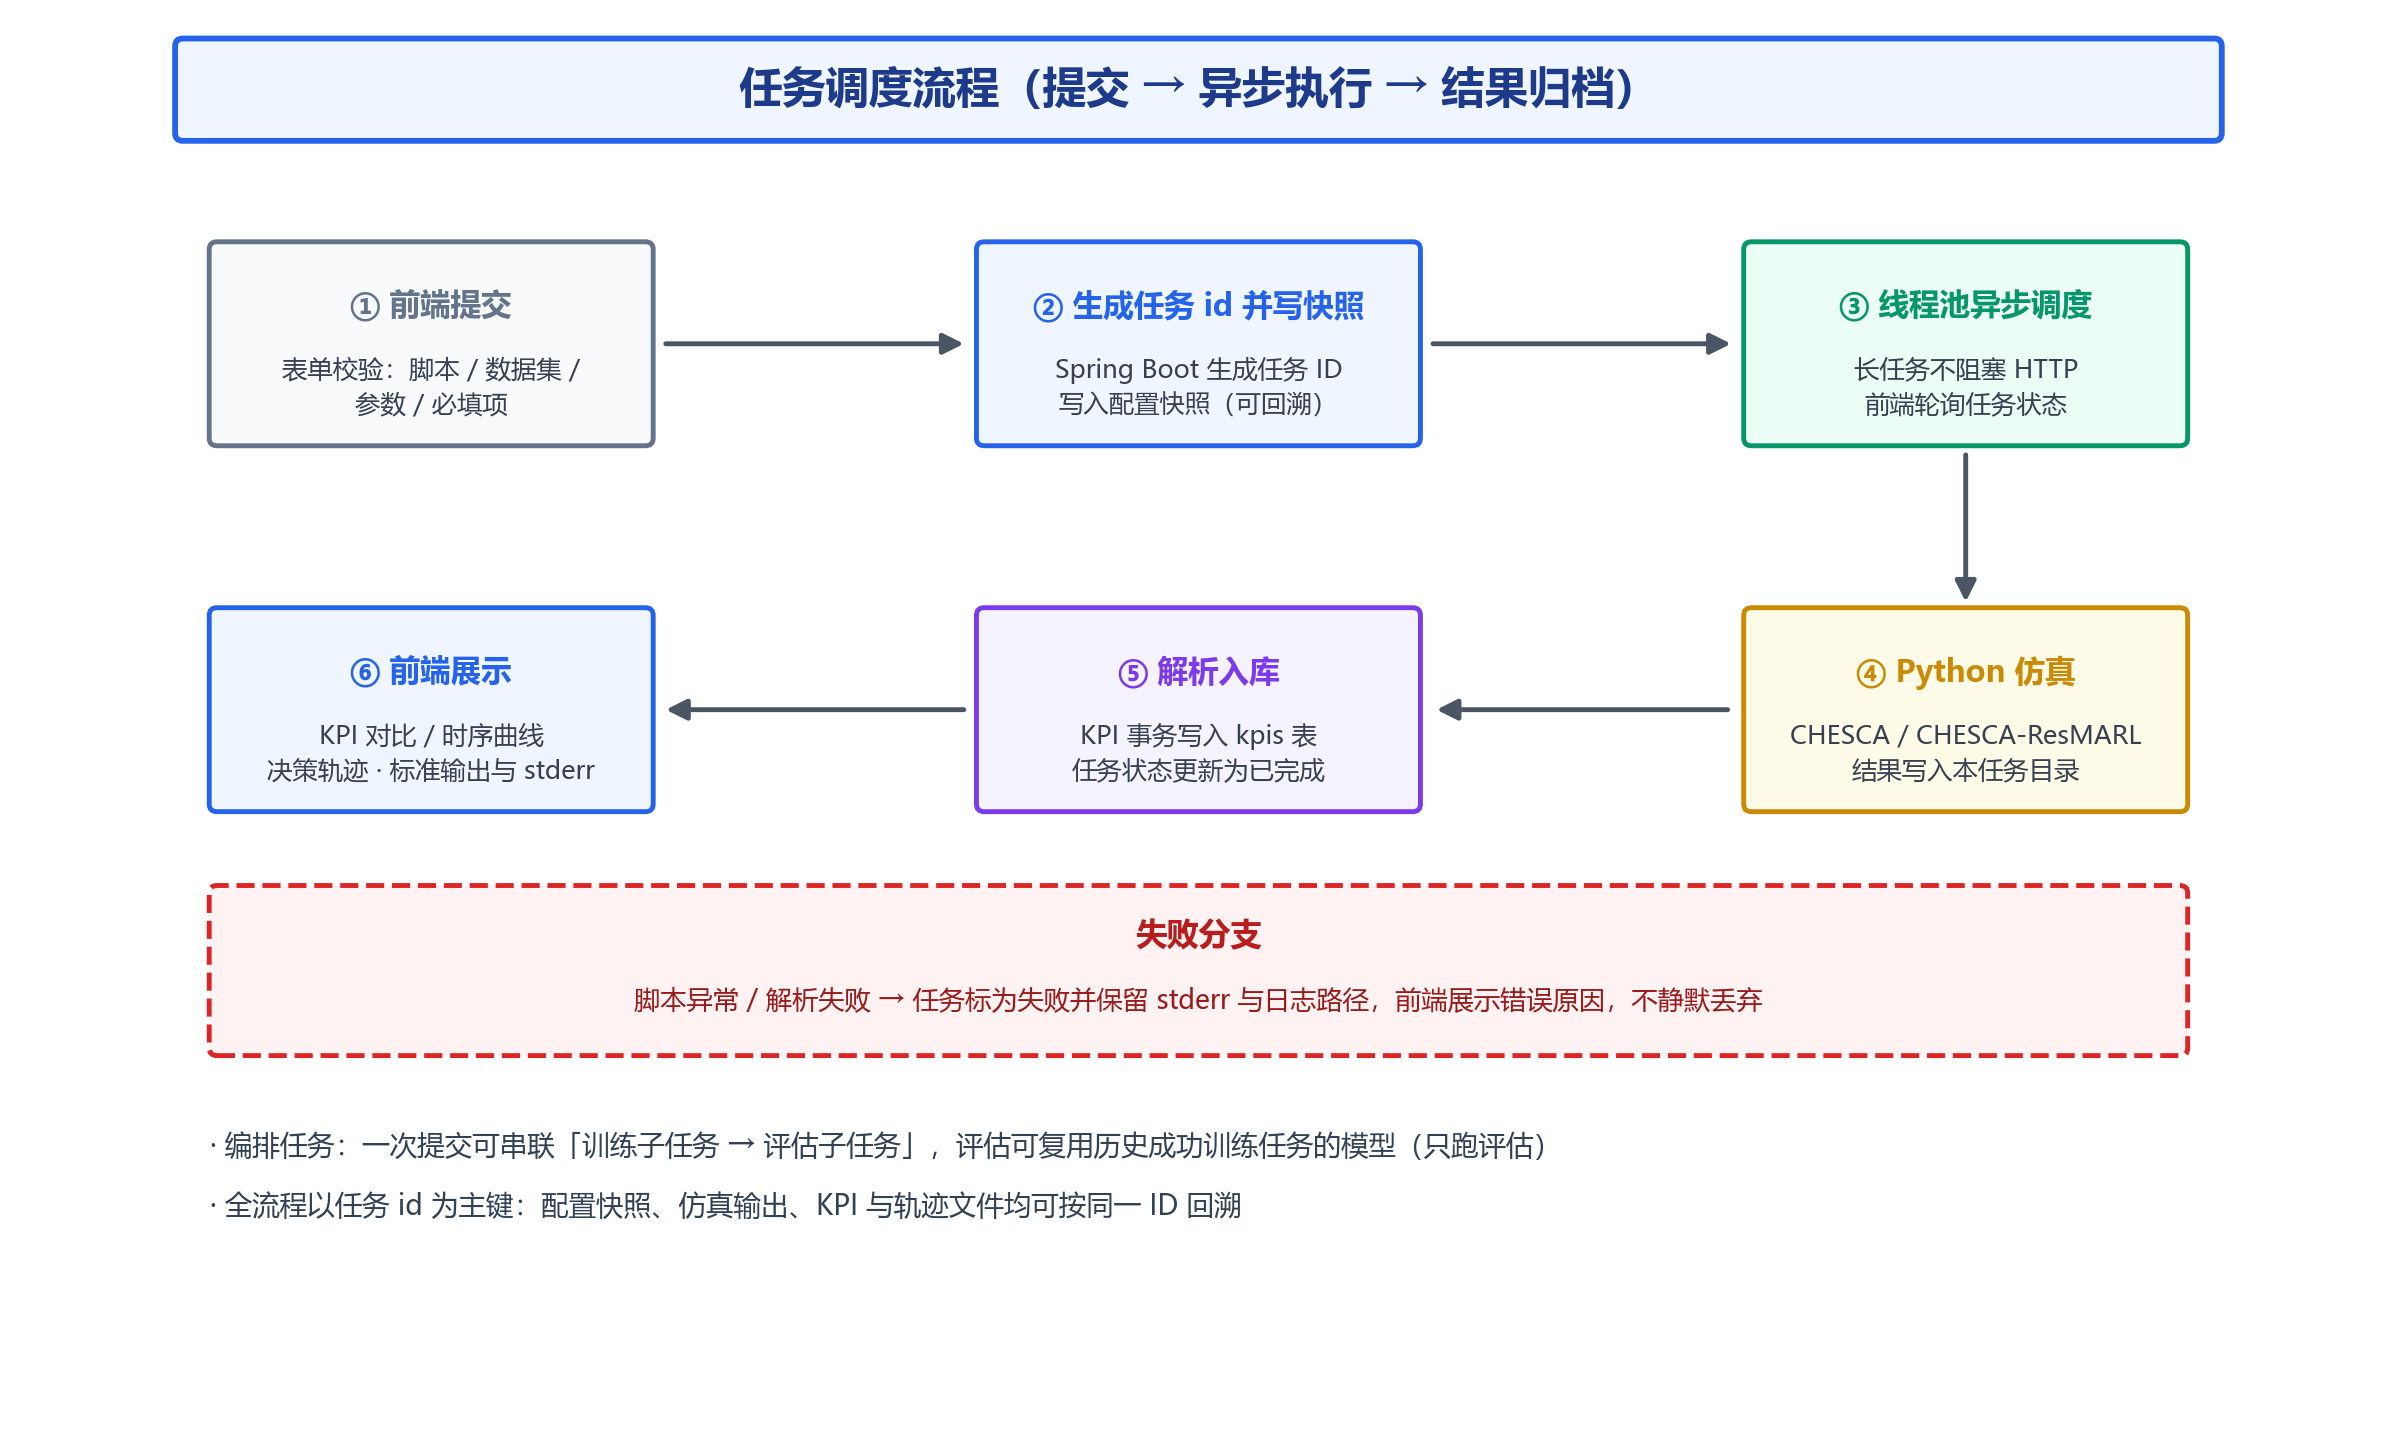
\includegraphics[width=0.90\textwidth]{./images/pictures/任务调度图.png}
    \centering\bicaption{任务调度图}{Task scheduling}
    \label{任务调度图}
\end{figure}

\begin{figure}[htb]
    \centering
    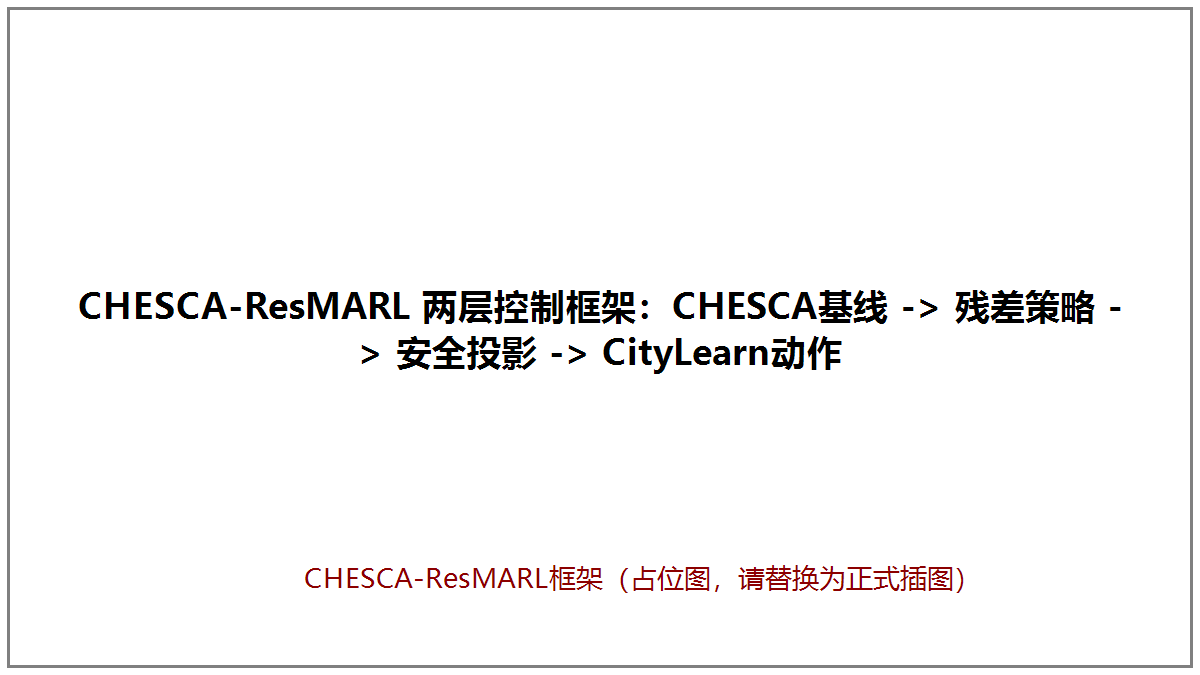
\includegraphics[width=0.85\textwidth]{./images/pictures/CHESCA-ResMARL框架.png}
    \centering\bicaption{CHESCA-ResMARL框架}{CHESCA-ResMARL framework}
    \label{CHESCA-ResMARL框架}
\end{figure}
残差合成过程如图\figref{残差合成图}所示。
\begin{figure}[htb]
    \centering
    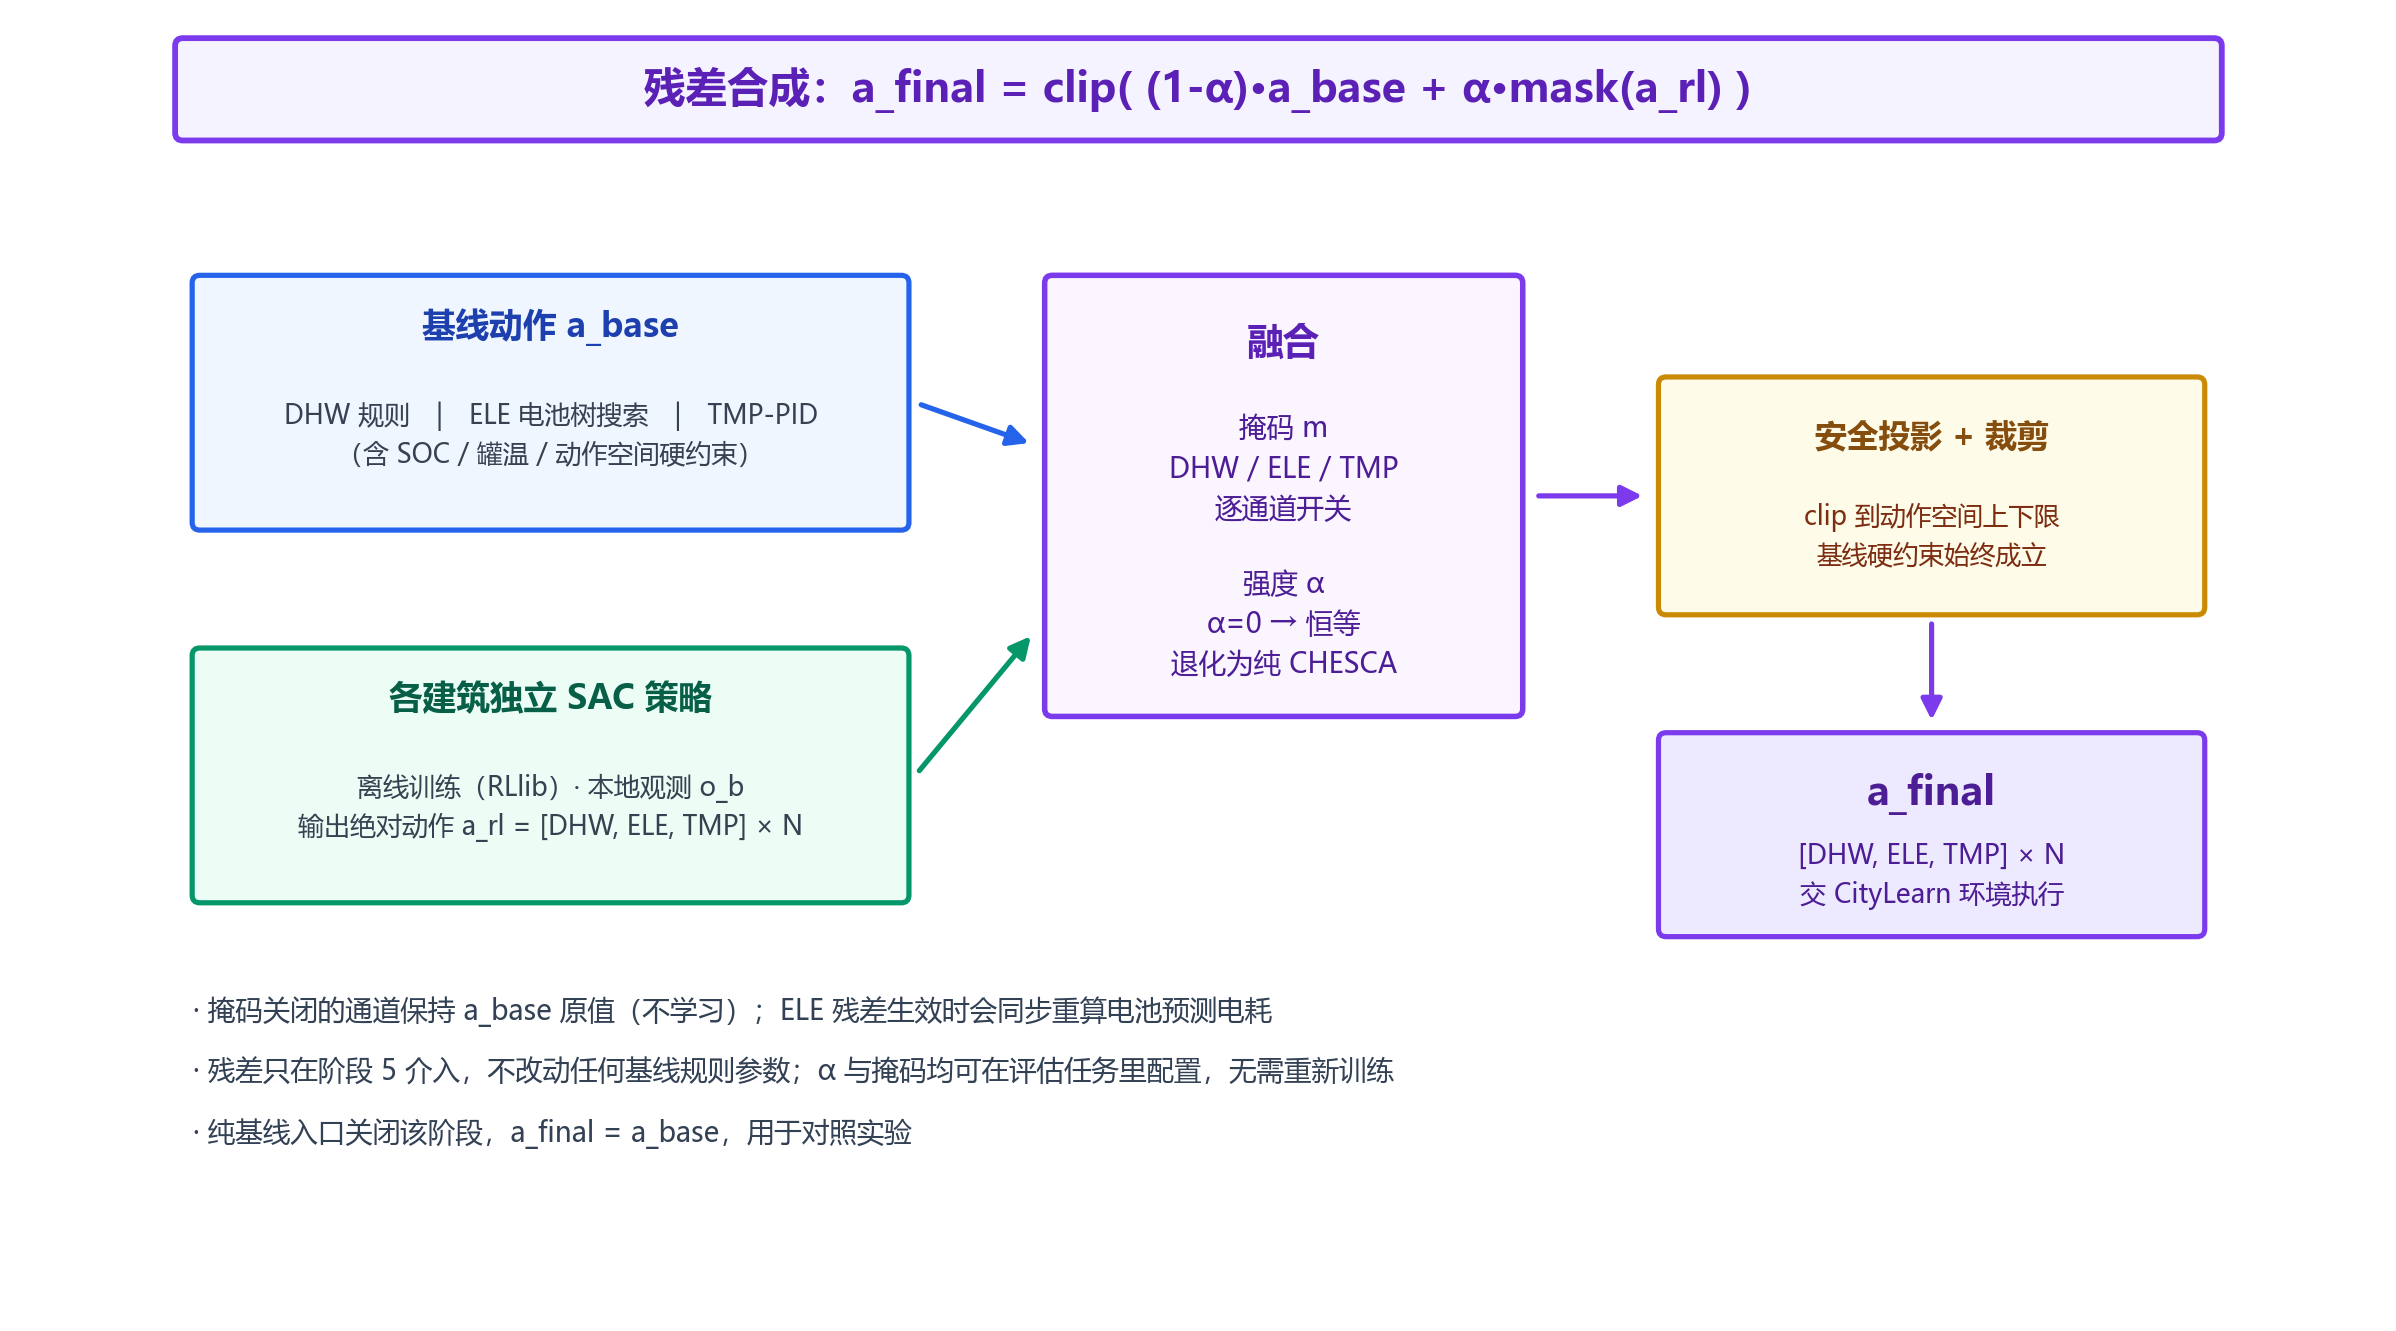
\includegraphics[width=0.92\textwidth]{./images/pictures/残差合成图.png}
    \centering\bicaption{残差合成图}{Residual fusion}
    \label{残差合成图}
\end{figure}

\section{前端系统功能介绍}
本节单独介绍前端系统功能，按``功能点+操作路径+界面截图''的方式组织，截图均取自平台实际运行界面。

\subsection{首页与导航}
功能：KPI卡片、新建任务快捷入口、通知入口。操作路径：登录进入首页，查看默认任务卡片，点击新建按钮跳转至配置页面。系统首页界面如图\ref{前端首页截图位}所示，包含导航栏、KPI卡片与新建任务快捷入口。
\begin{figure}[htb]
    \centering
    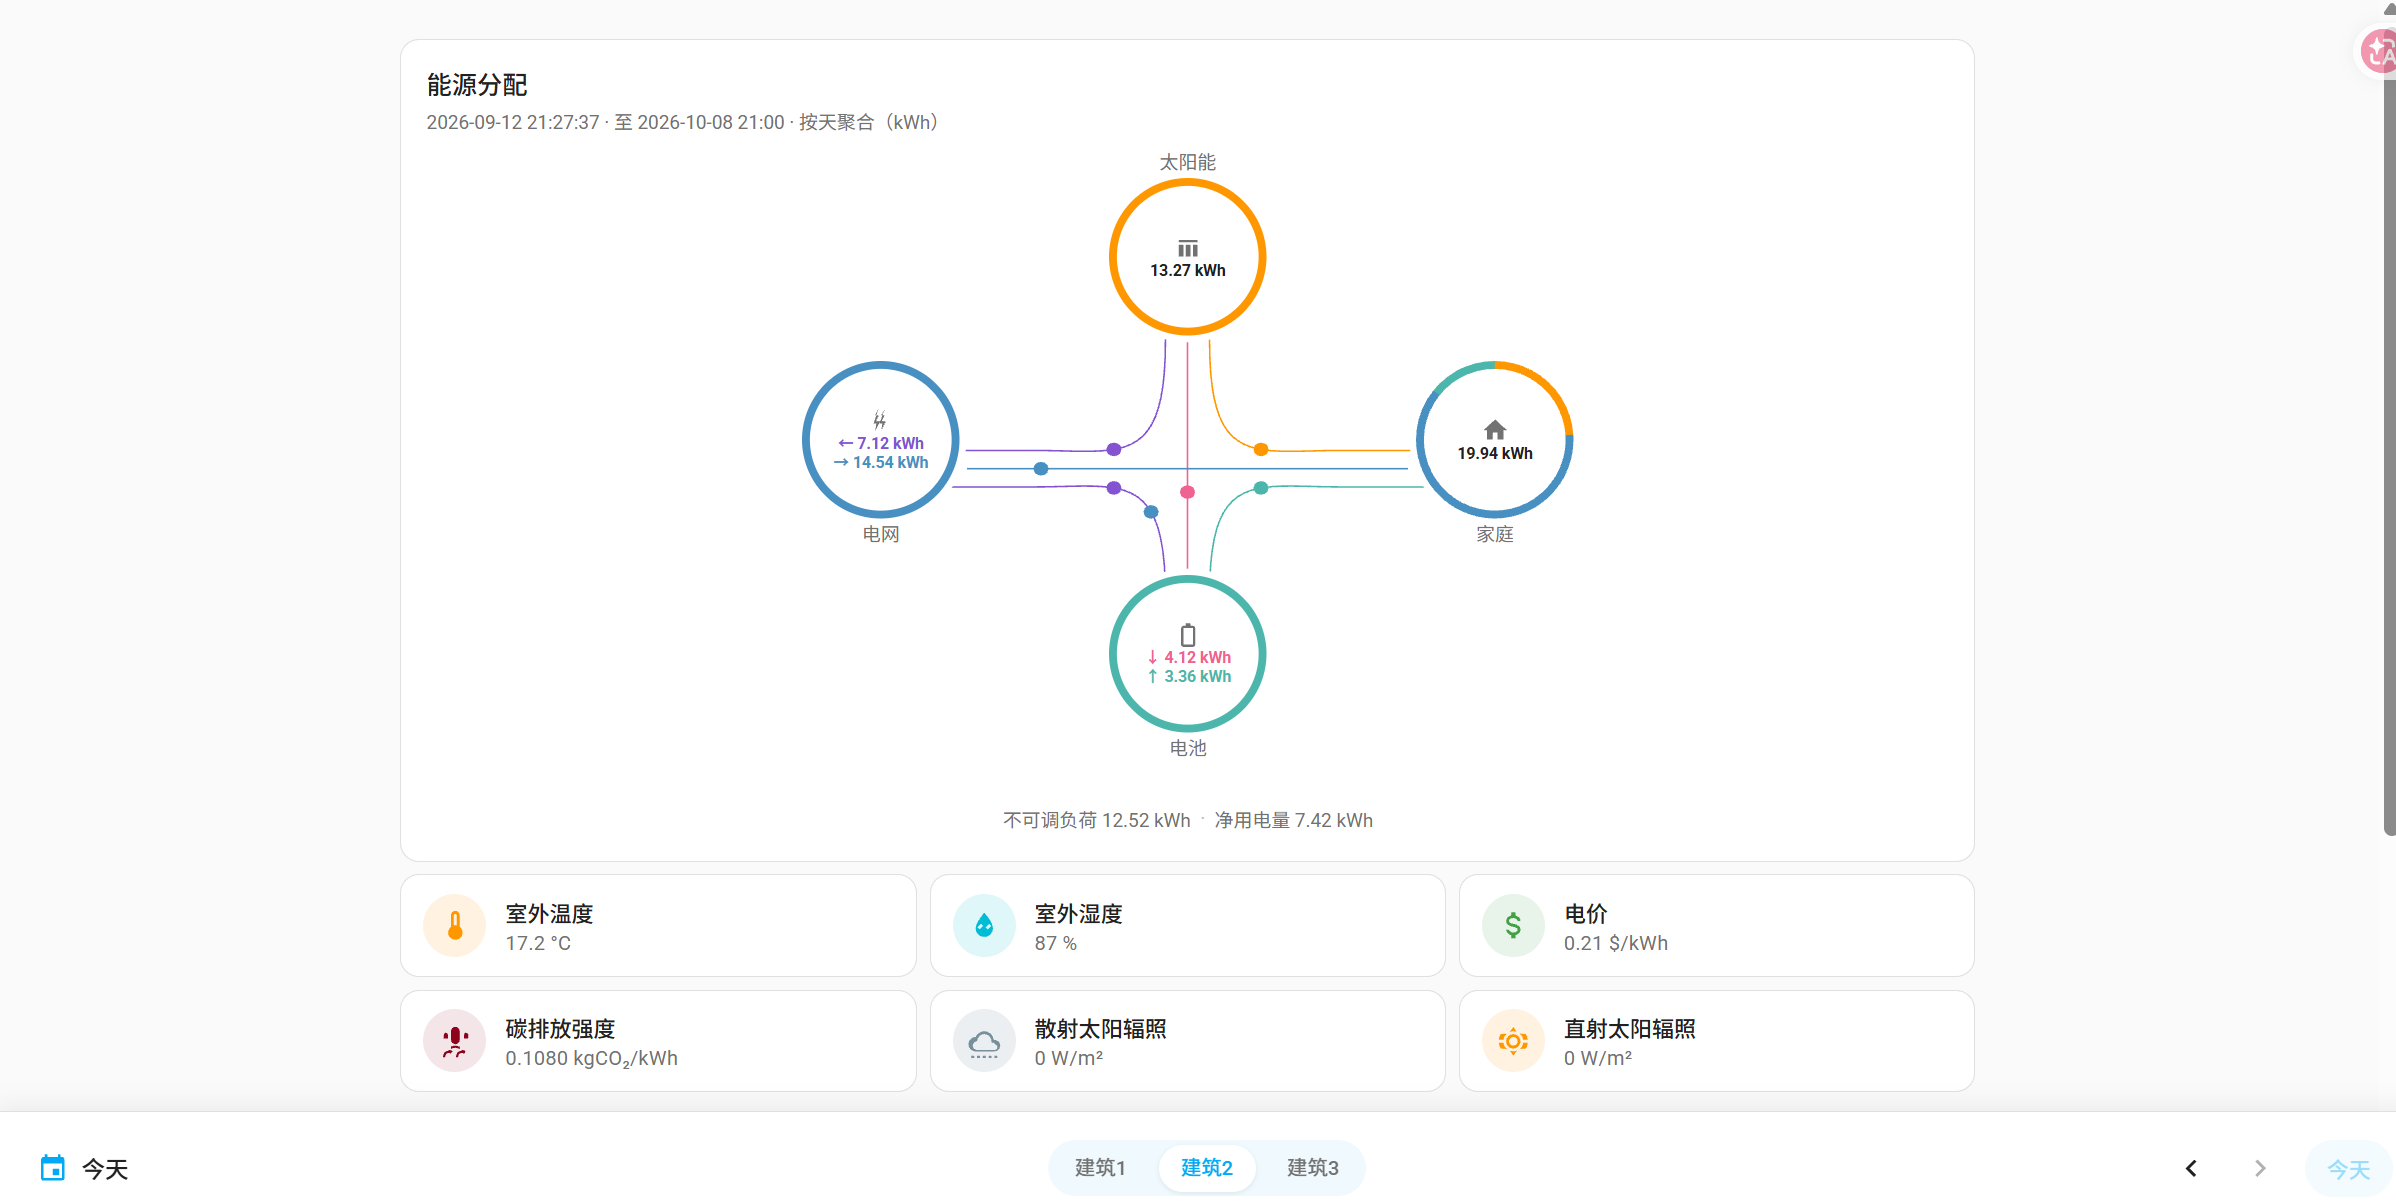
\includegraphics[width=0.85\textwidth]{./images/image/首页.jpg}
    \centering\bicaption{系统首页界面}{Frontend home}
    \label{前端首页截图位}
\end{figure}

\subsection{模型配置与任务提交}
功能：选择控制器、数据集、步数、残差系数、掩码、安全开关与模型文件，表单校验不通过时不发送请求。操作路径：在模型配置页填写参数并提交，在任务列表查看状态。算法配置界面如图\ref{前端配置截图位}所示，包含控制器、数据集、步数、残差系数、通道掩码、安全开关与模型文件等参数项，表单校验不通过时不发送请求。
\begin{figure}[htb]
    \centering
    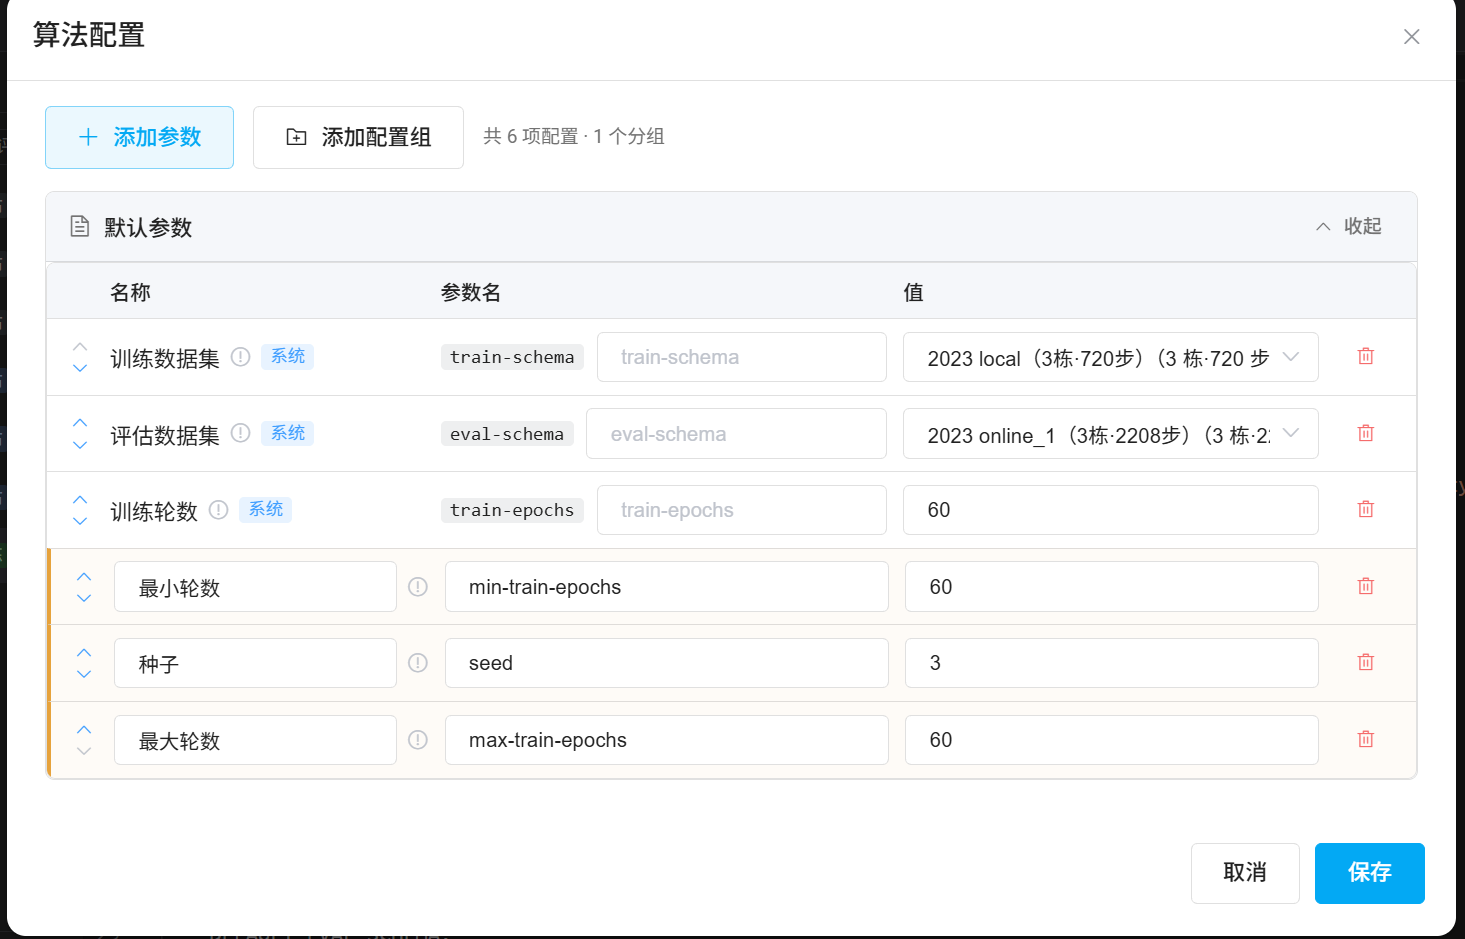
\includegraphics[width=0.85\textwidth]{./images/image/算法配置页.jpg}
    \centering\bicaption{算法配置页面}{Algorithm configuration page}
    \label{前端配置截图位}
\end{figure}

\subsection{能源分析与KPI对比}
功能：多任务KPI柱状图与雷达图、时序折线、任务检索。操作路径：在能源分析页输入任务标识，切换柱状/雷达/折线视图，对比无控制、CHESCA与残差策略。KPI指标对比界面如图\ref{前端KPI截图位}所示；原始数据查看页面支持按任务导出CSV时序数据，如图\ref{KPI对比图位}所示。
\begin{figure}[htb]
    \centering
    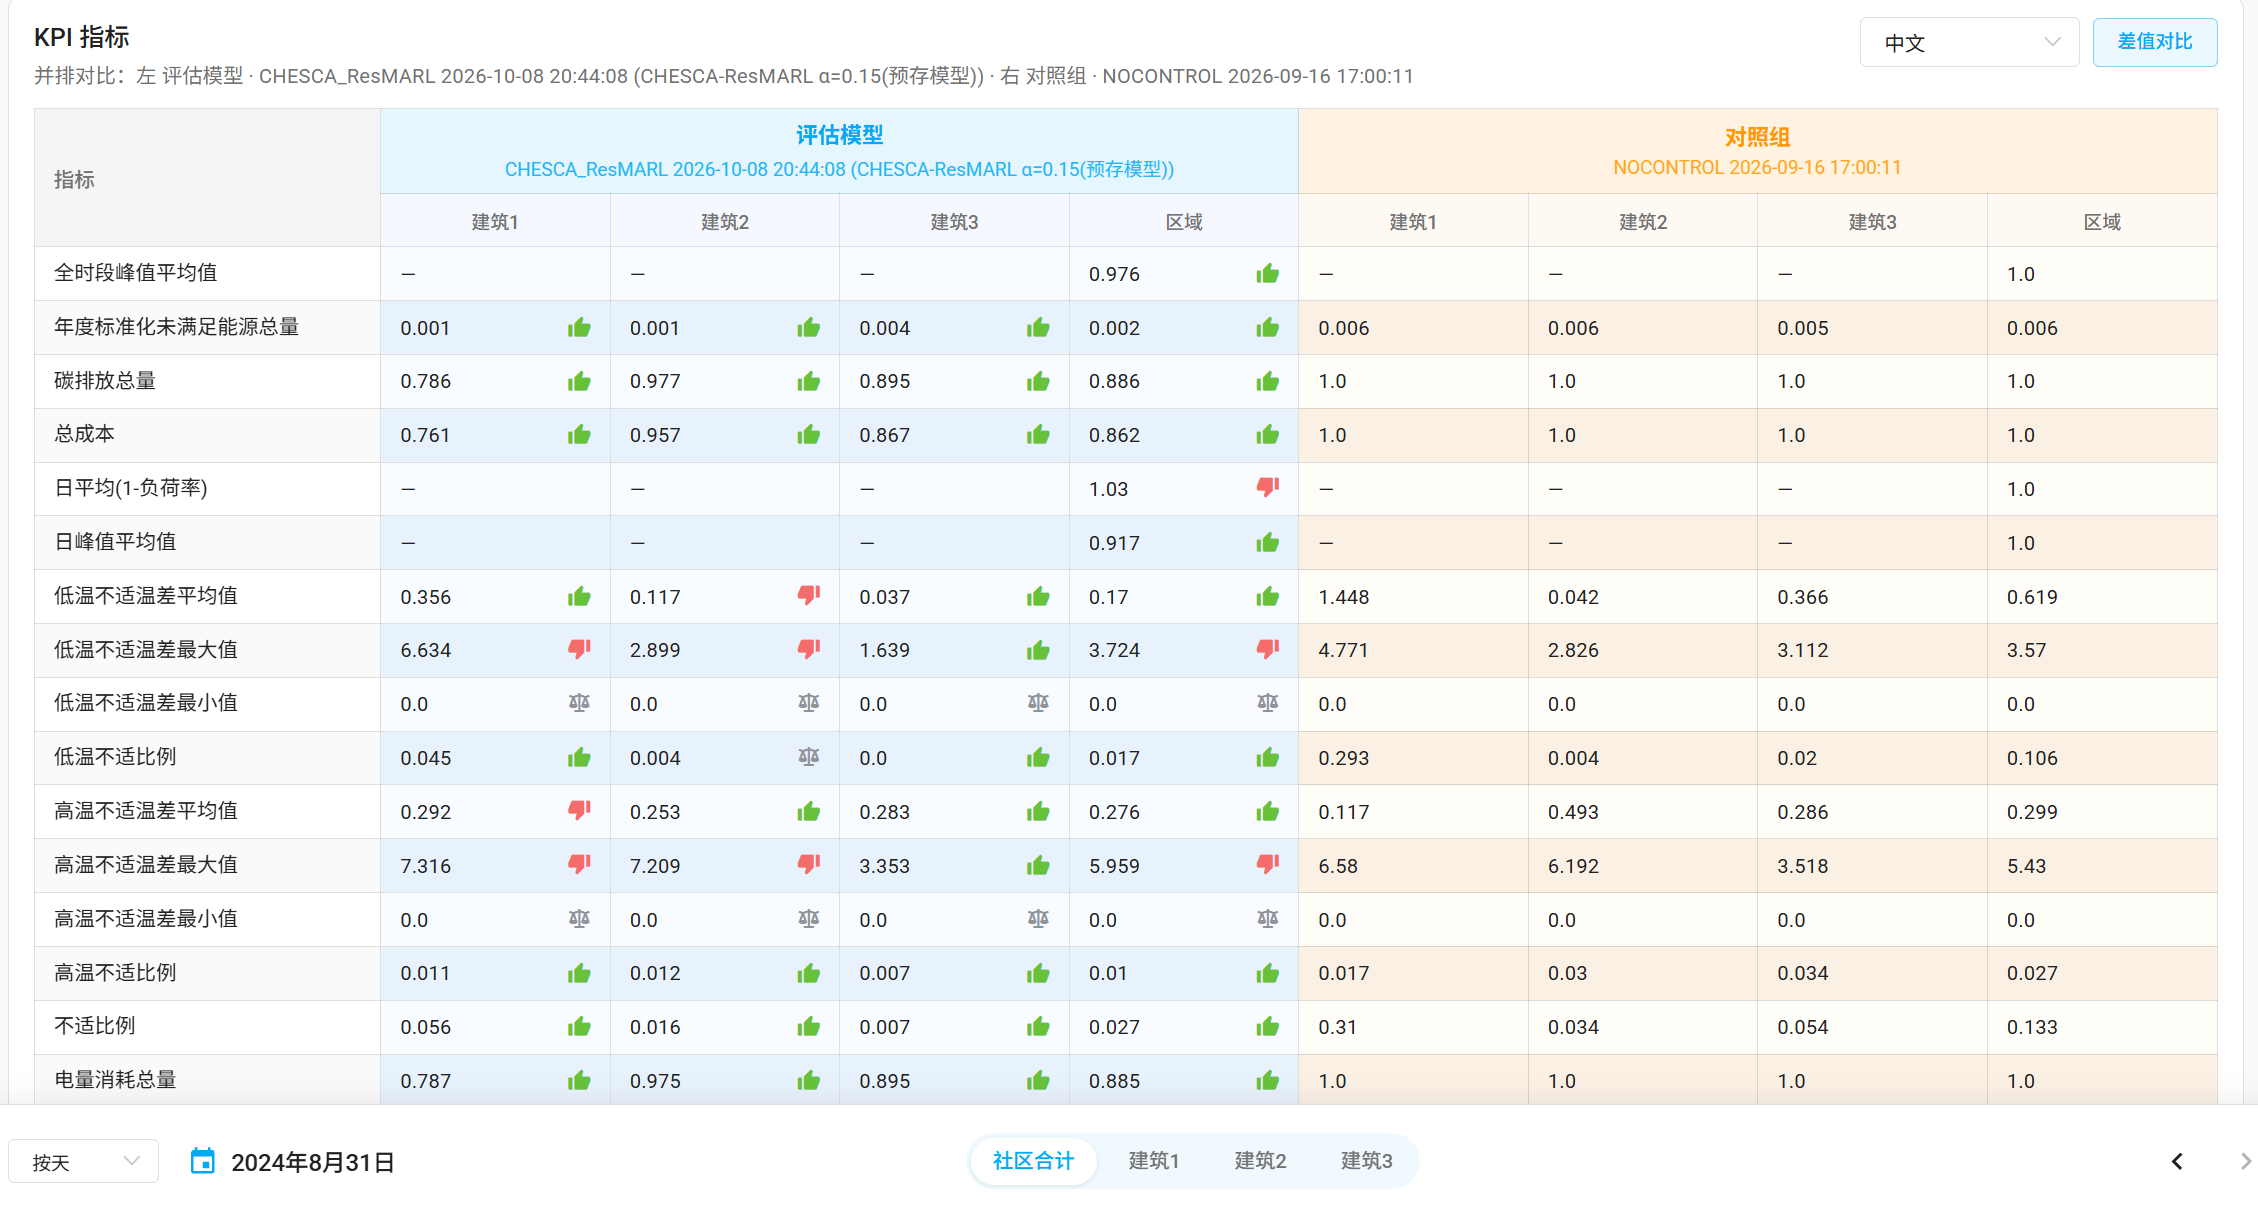
\includegraphics[width=0.85\textwidth]{./images/image/指标对比.jpg}
    \centering\bicaption{KPI指标对比页面}{KPI comparison}
    \label{前端KPI截图位}
\end{figure}
\begin{figure}[htb]
    \centering
    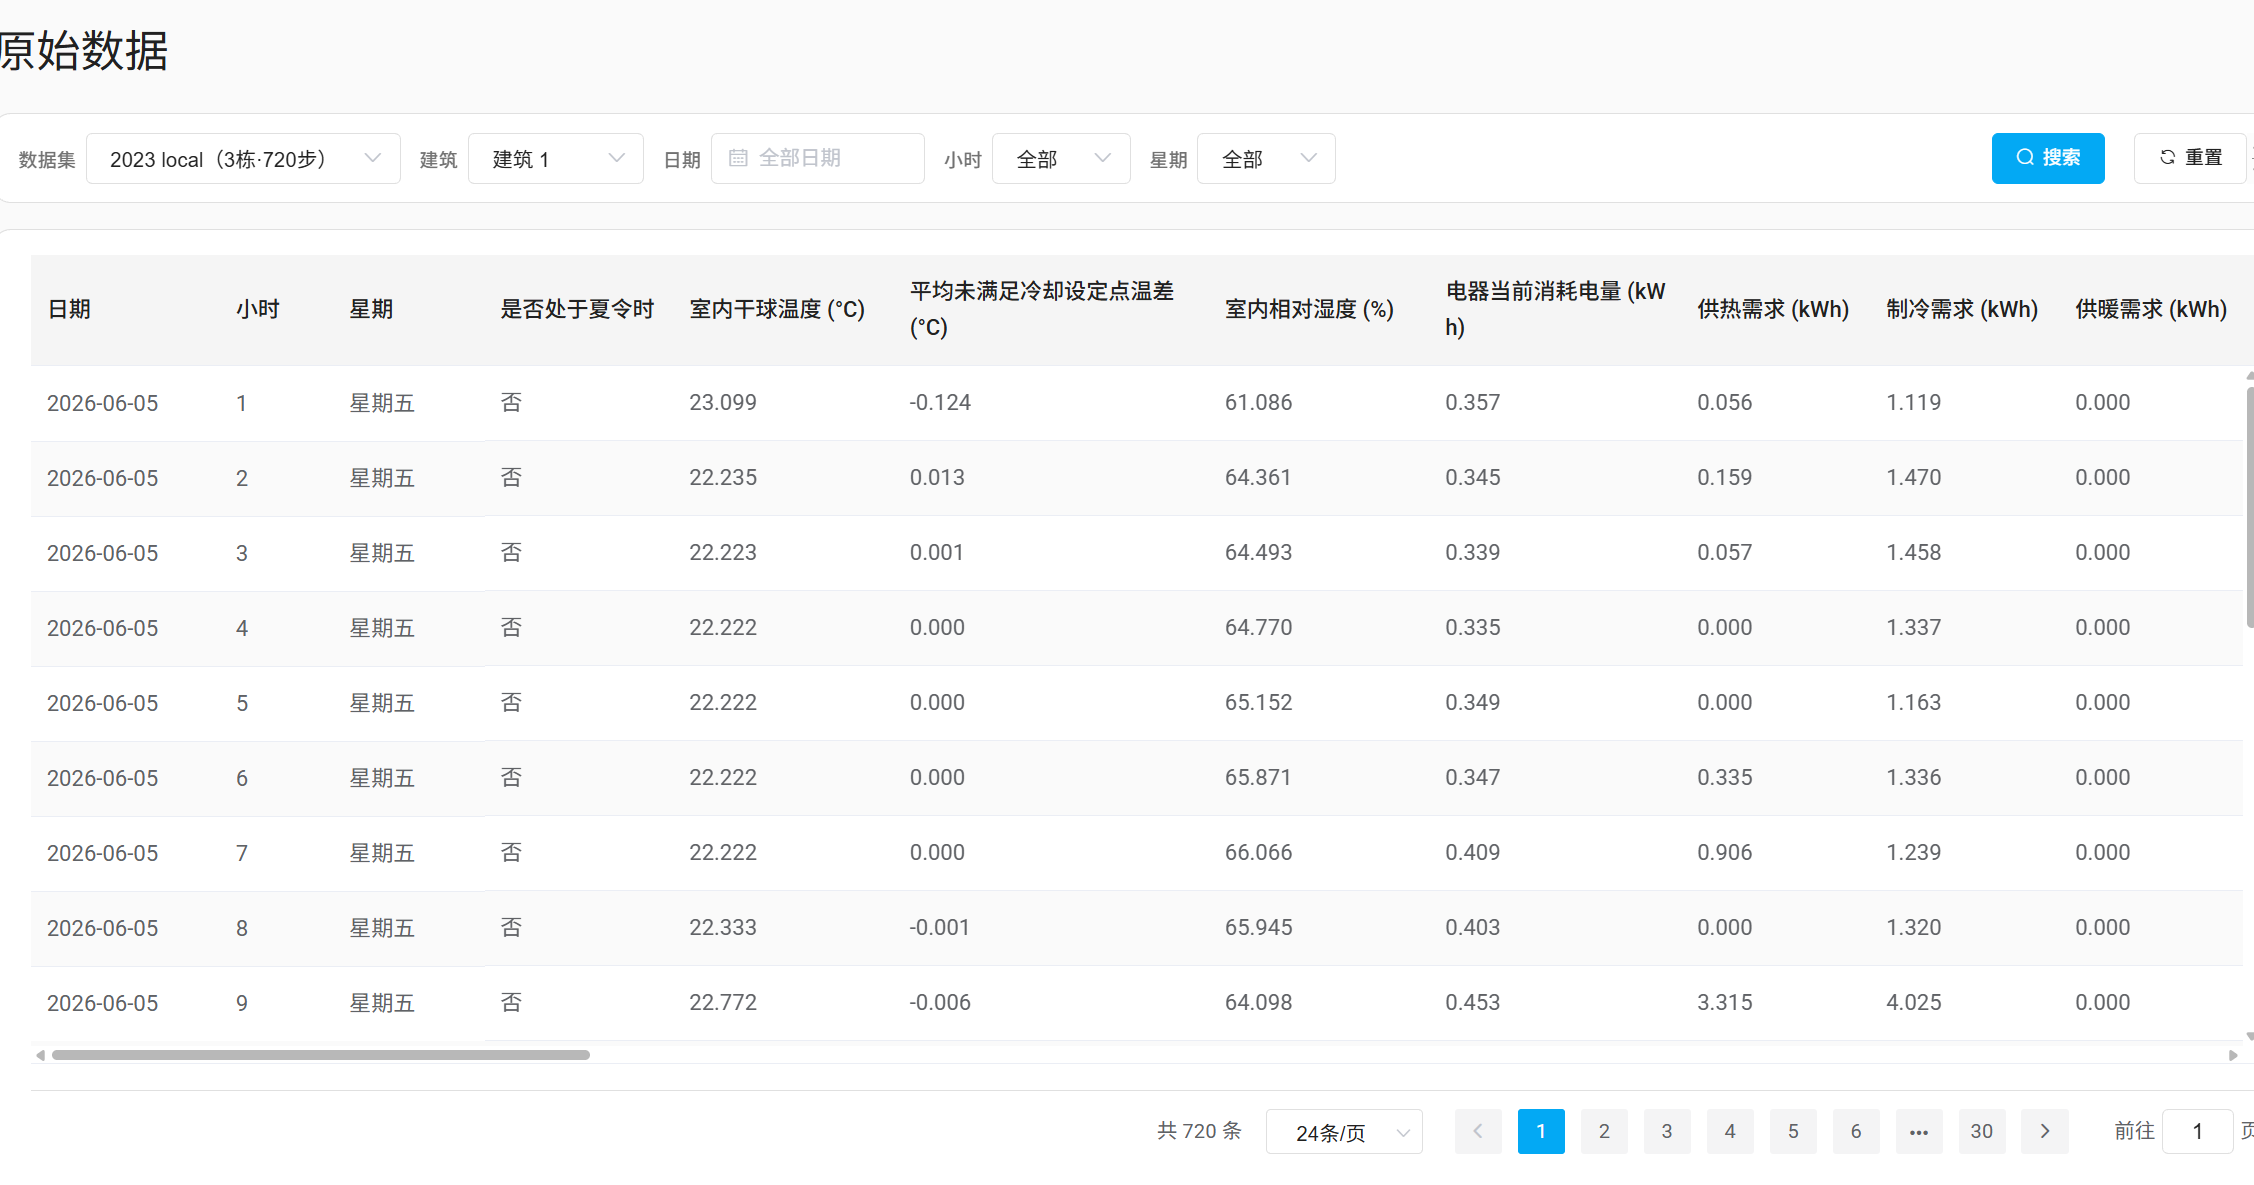
\includegraphics[width=0.85\textwidth]{./images/image/原始数据页.jpg}
    \centering\bicaption{原始数据查看页面}{Raw time-series data page}
    \label{KPI对比图位}
\end{figure}

\subsection{决策轨迹与残差查看}
功能：按时间步查看基线、残差、掩码、投影、SOC与舒适度状态，定位峰值时段。操作路径：在决策轨迹页输入任务标识与时间步，查看残差是否被安全层裁剪。决策轨迹页的环境状态面板如图\ref{前端轨迹截图位}与图\ref{环境状态动作截图位}所示，可查看室温、SOC与电价等状态量随时间步的变化。
\begin{figure}[htb]
    \centering
    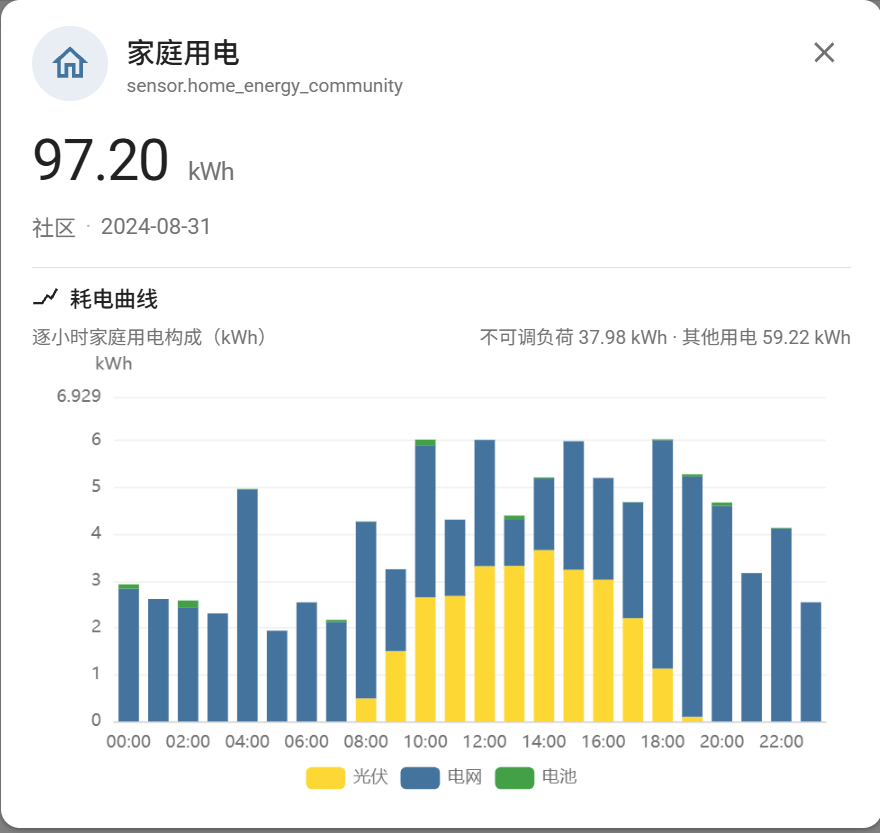
\includegraphics[width=0.85\textwidth]{./images/image/环境状态1.jpg}
    \centering\bicaption{决策轨迹环境状态（室温与SOC）}{Decision trace: temperature and SOC}
    \label{前端轨迹截图位}
\end{figure}
\begin{figure}[htb]
    \centering
    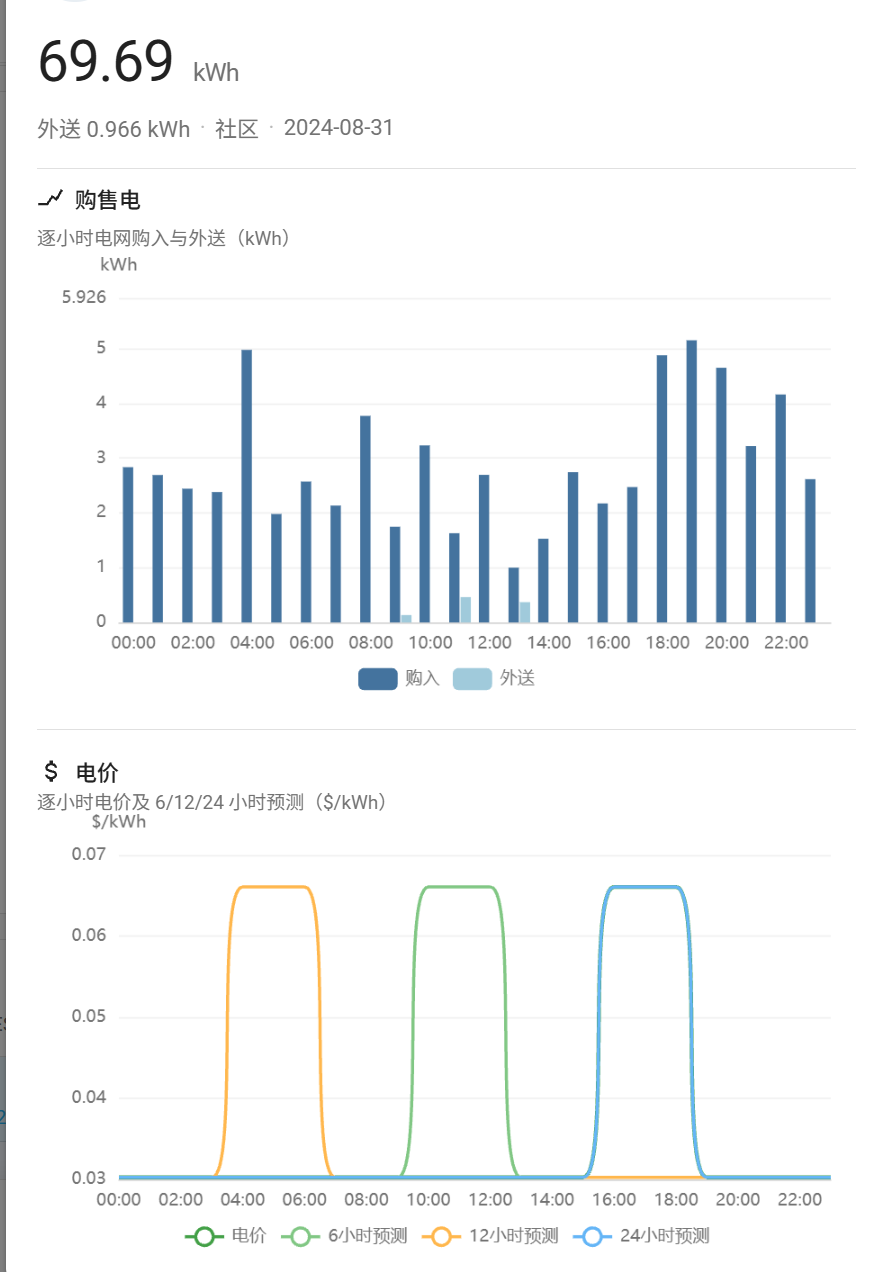
\includegraphics[width=0.85\textwidth]{./images/image/环境状态2-电价.jpg}
    \centering\bicaption{决策轨迹环境状态（电价）}{Decision trace: electricity price}
    \label{环境状态动作截图位}
\end{figure}

\subsection{其他页面与自动生成流程}
任务列表页面提供任务分页查询、进度跟踪与日志查看，菜单入口受权限控制；算法参数配置页面以分组表单维护各算法参数并内置在线代码编辑器，脚本编辑界面如图\ref{代码编辑器}所示；用户管理页面维护用户与角色；登录页面完成身份认证与跳转。此外，系统还提供了残差系数敏感性分析、预测误差展示与各通道残差分布展示等辅助视图。任务管理自动化流程如图\ref{自动可视化流程占位}所示，覆盖从数据集准备、训练、评估到指标入库的完整链路；残差调优流程以示意图形式给出。
\begin{figure}[htb]
    \centering
    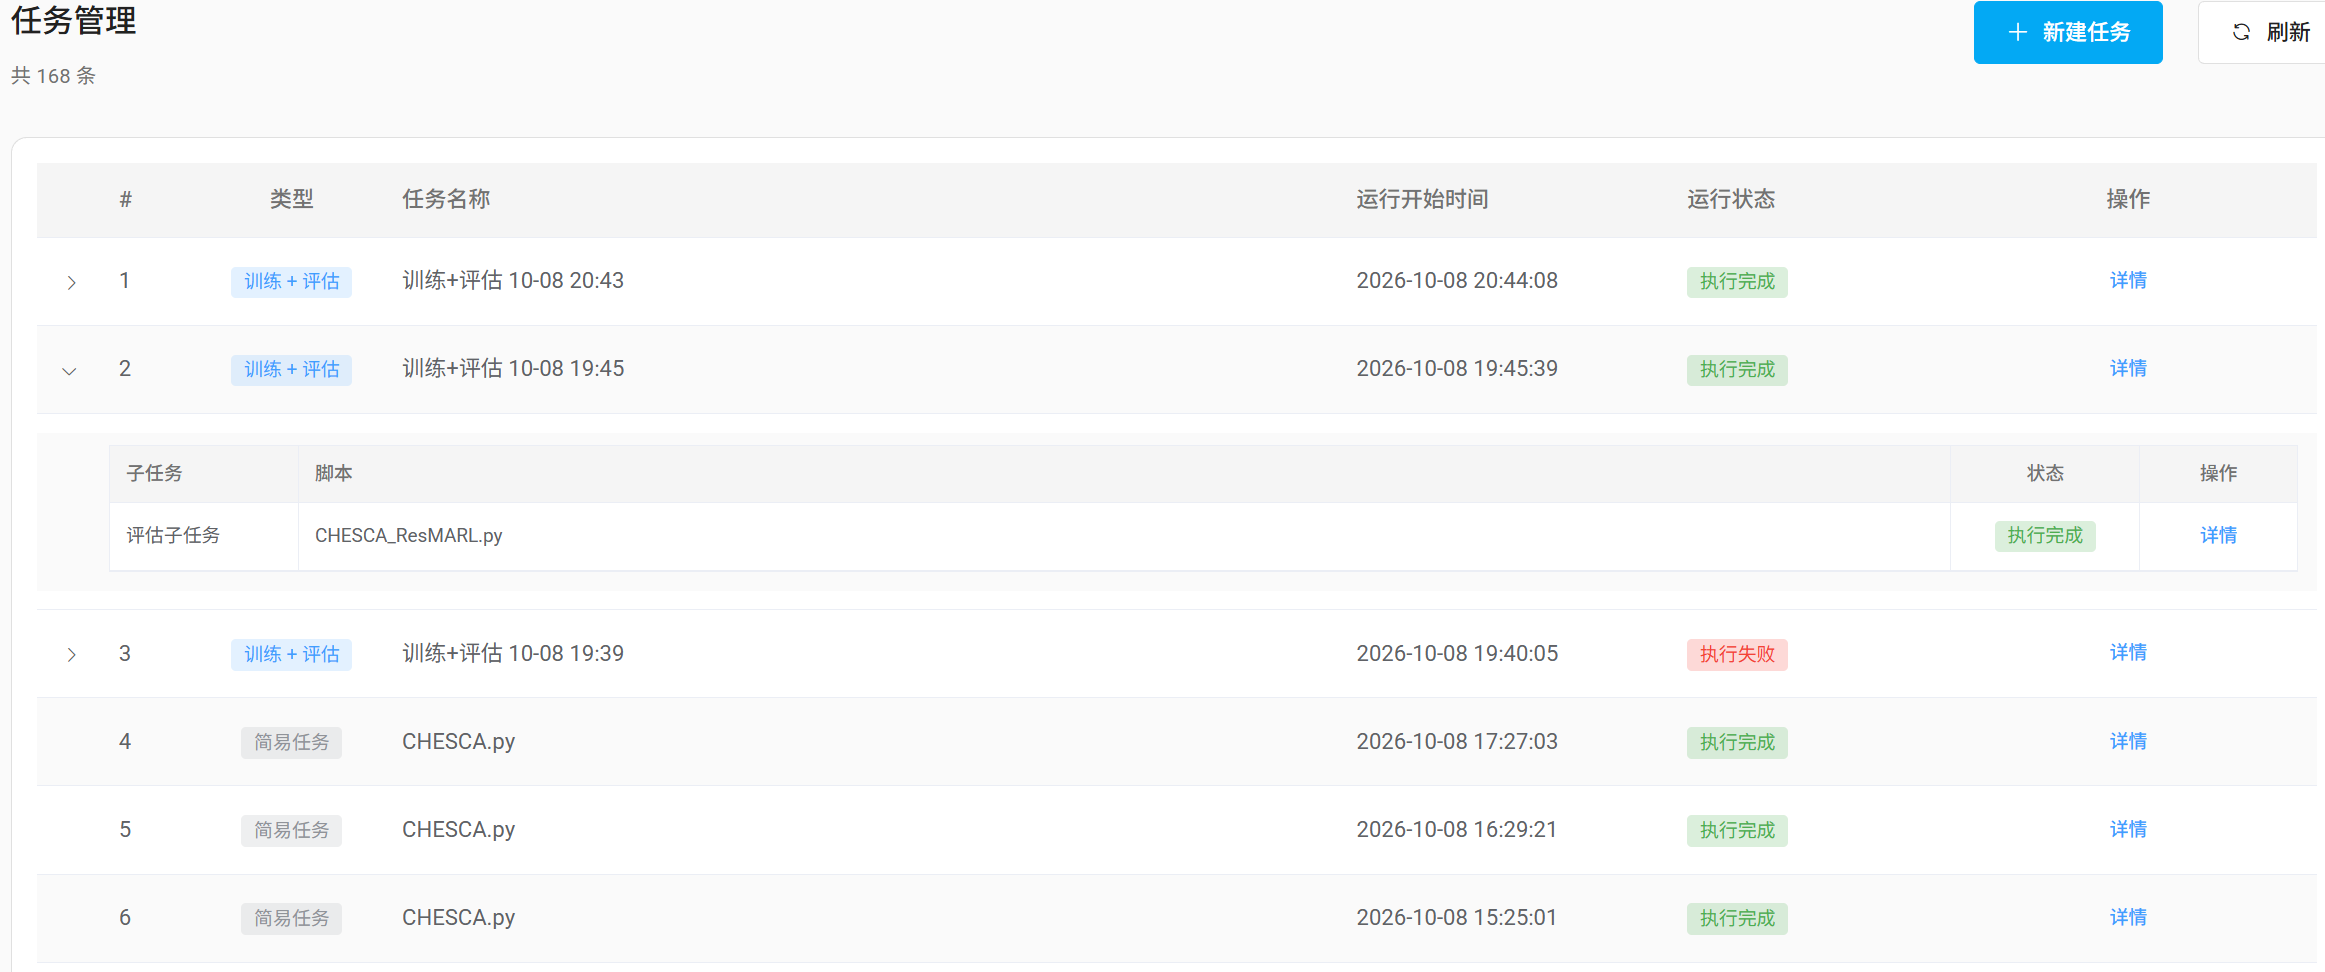
\includegraphics[width=0.8\textwidth]{./images/image/任务管理自动化流程.jpg}
    \centering\bicaption{任务管理自动化流程}{Task management automation pipeline}
    \label{自动可视化流程占位}
\end{figure}
\begin{figure}[htb]
    \centering
    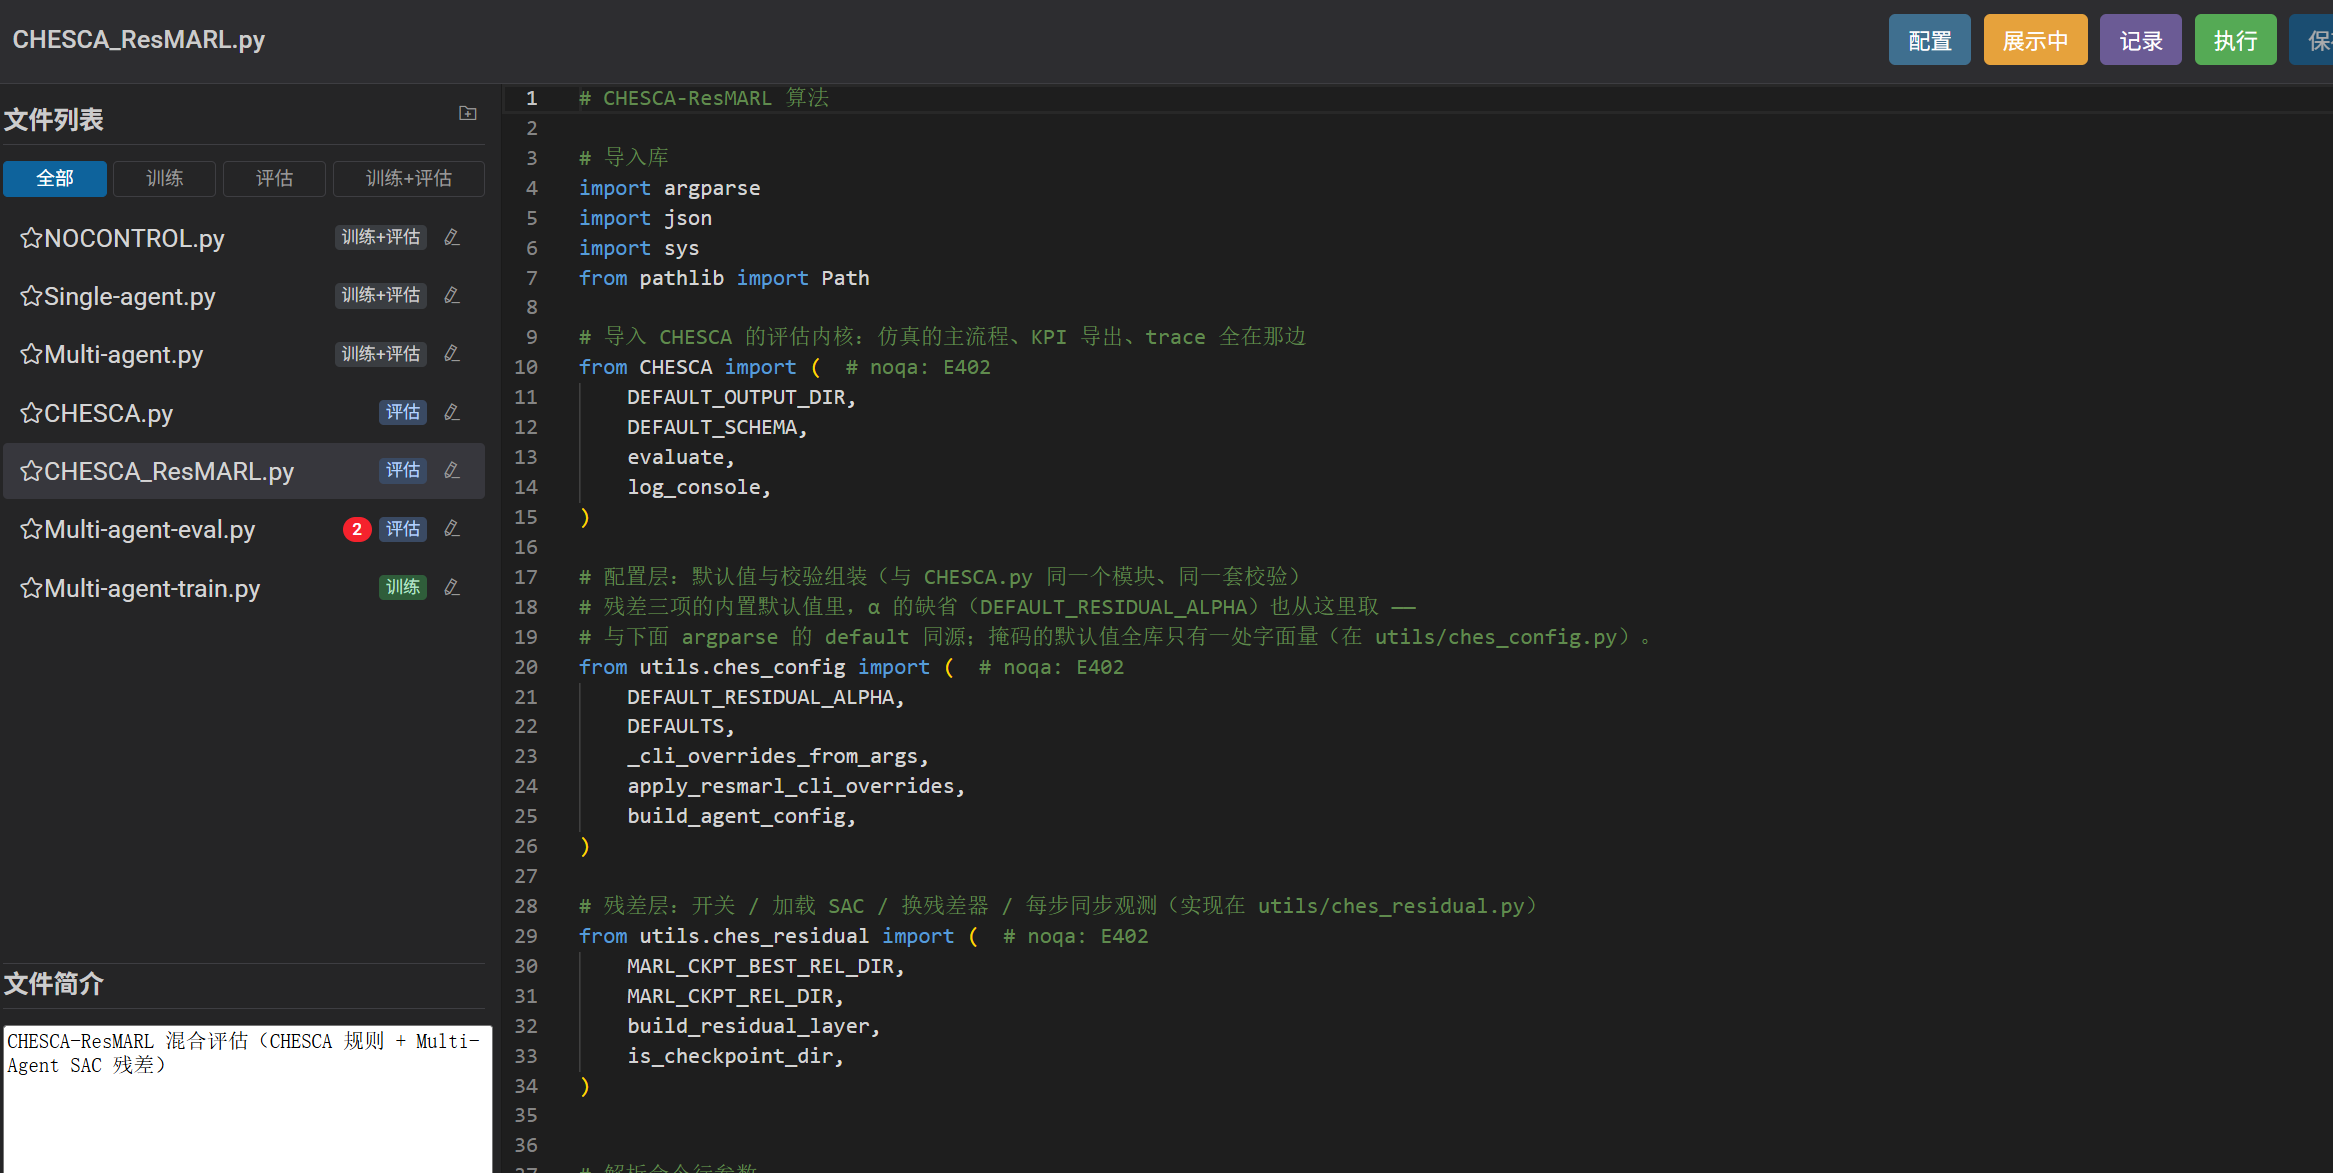
\includegraphics[width=0.85\textwidth]{./images/image/代码编辑器.jpg}
    \centering\bicaption{算法参数配置与脚本编辑界面}{Algorithm parameter configuration and script editing}
    \label{代码编辑器}
\end{figure}
\begin{figure}[htb]
    \centering
    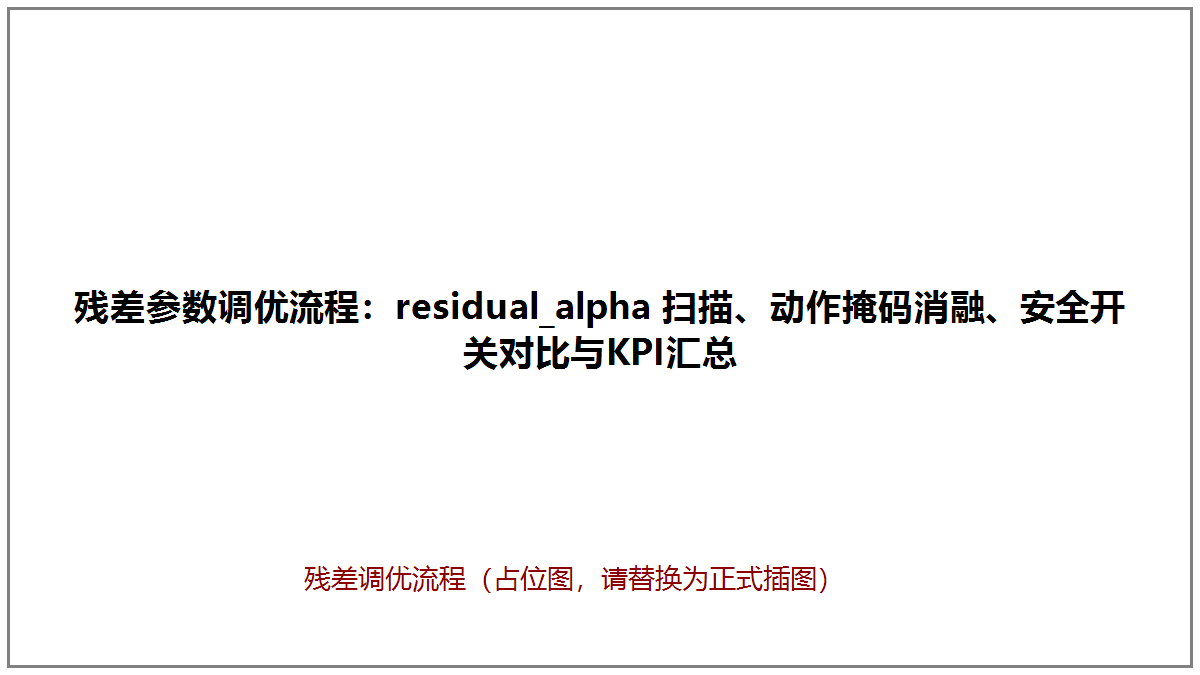
\includegraphics[width=0.8\textwidth]{./images/pictures/残差调优流程.png}
    \centering\bicaption{残差调优流程}{Residual tuning workflow}
    \label{残差调优流程占位}
\end{figure}

\section{本章小结}
本章将系统设计落地为具体实现：页面部分阐述布局与校验逻辑，日志部分说明当前组合方案与ELK备选，存储部分介绍五组数据表与索引设计，调度部分说明任务标识贯通全链路的机制，前端部分单列章节介绍界面功能。下一章将通过Postman契约测试、功能用例与CityLearn消融实验对上述内容进行验证。

\chapter{实验与结果分析}

\section{系统测试与测试用例}
\subsection{接口测试}
本系统采用前后端分离设计模式，为确保测试过程的高效性与严谨性，采用契约测试方法验证接口数据交换的准确性和后端逻辑的正确性。测试重点覆盖数据集列表、算法脚本列表、任务创建、任务状态、KPI查询与决策轨迹查询接口。每个接口均验证正常请求、缺失参数、非法参数、资源不存在和任务失败等场景。

前后端接口文档按照统一JSON协议维护，任务创建接口返回唯一\texttt{taskId}，状态查询接口返回0（执行中）、1（完成）、2（失败），KPI接口在任务完成后返回聚合指标，轨迹接口返回CSV/JSON文件索引。接口测试应使用Apifox或Postman保存请求参数与响应样例，确保后续论文结果可复现。

\begin{table}[h!]
    \centering\bicaption{接口测试用例}{API test cases}
    \label{tab:api-cases}
    \begin{tabular}{P{5em}P{8em}P{10em}P{8em}}
        \toprule
        编号 & 用例名称 & 操作步骤 & 预期结果 \\\midrule
        1 & 数据集查询 & 请求已启用schema列表 & 返回名称、步数与兼容性 \\
        2 & 任务创建 & 提交CHESCA有效参数 & 返回唯一taskId \\
        3 & 参数校验 & ResMARL不填checkpoint & 拒绝提交并提示原因 \\
        4 & 状态查询 & 按taskId轮询任务 & 状态正确更新 \\
        5 & KPI查询 & 查询已完成任务 & 返回完整KPI记录 \\
        6 & 非法任务 & 查询不存在taskId & 返回资源不存在 \\
        \bottomrule
    \end{tabular}
\end{table}

\subsection{功能测试}
功能测试遵循黑盒测试原则，重点覆盖登录、数据集管理、算法选择、任务提交、任务状态展示、KPI分析与决策轨迹展示。测试结果应以实际运行记录为准，本文不将尚未完成的功能描述为已通过。

\begin{table}[h!]
    \centering\bicaption{平台功能测试用例}{Platform functional test cases}
    \label{tab:function-cases}
    \begin{tabular}{P{5em}P{8em}P{10em}P{8em}}
        \toprule
        编号 & 用例名称 & 操作步骤 & 预期结果 \\\midrule
        1 & 登录系统 & 输入正确账号密码 & 进入有权限页面 \\
        2 & 选择数据集 & 选择schema并查看元数据 & 显示建筑数和步数 \\
        3 & 提交CHESCA & 配置算法并提交任务 & 任务进入执行状态 \\
        4 & 提交ResMARL & 配置checkpoint与残差参数 & 任务正常执行 \\
        5 & 查看KPI & 打开已完成任务 & 显示表格和图表 \\
        6 & 查看轨迹 & 定位指定时间步 & 显示动作与投影结果 \\
        \bottomrule
    \end{tabular}
\end{table}

\subsection{非功能性测试}
非功能性测试包括安全性、兼容性、稳定性与可维护性测试。安全性测试关注SQL注入、XSS、越权访问、恶意路径与非法文件上传；兼容性测试关注Chrome、Edge和Firefox浏览器中的页面布局与ECharts渲染；稳定性测试关注长时间仿真、任务失败重试和结果目录隔离；可维护性测试关注日志是否包含taskId、配置快照与错误堆栈。

\begin{table}[h!]
    \centering\bicaption{非功能性测试用例}{Non-functional test cases}
    \label{tab:nonfunctional-cases}
    \begin{tabular}{P{5em}P{8em}P{10em}P{8em}}
        \toprule
        编号 & 用例名称 & 操作步骤 & 预期结果 \\\midrule
        1 & SQL注入防护 & 在筛选参数输入恶意字符串 & 返回校验错误 \\
        2 & XSS防护 & 提交包含脚本的反馈内容 & 内容被转义 \\
        3 & 路径安全 & 提交相对路径和绝对路径 & 禁止越权读取 \\
        4 & 任务隔离 & 同时提交两个任务 & 结果目录互不覆盖 \\
        5 & 浏览器兼容 & 使用Chrome、Edge、Firefox访问 & 页面正常渲染 \\
        6 & 长任务稳定性 & 执行长周期schema & 状态持续可查询 \\
        \bottomrule
    \end{tabular}
\end{table}

\section{算法测试}
本文以CityLearn建筑群能源管理任务为实验环境，比较NOCONTROL、CHESCA与CHESCA-ResMARL的控制效果。实验数据由\texttt{citylearn\_challenge\_2023\_phase\_2\_local\_evaluation}及2026兼容schema构建，评价指标包括Total Cost、Carbon Emissions、Peak、Ramping、Discomfort、Electricity Consumption、Renewable Supplied Energy与Zero Net Energy。所有实验记录算法名称、数据集schema、步数、残差参数、checkpoint和输出目录。

实验过程分为四步：首先运行NOCONTROL得到无控制参考；其次运行纯CHESCA验证基线链路；再次运行\texttt{residual\_alpha=0}的ResMARL配置验证混合入口能够退化为基线；最后在不同残差幅度、动作掩码和安全后处理开关下运行完整策略。每组正式实验至少使用5个随机种子，并报告均值、标准差和置信区间。

\section{阶段性实验结果}
当前项目的\texttt{ablation\_results/ablation\_summary.json}包含720步、单次运行的阶段性结果。纯CHESCA的社区KPI为：\texttt{all\_time\_peak\_average}=0.832，\texttt{carbon\_emissions\_total}=0.407，\texttt{cost\_total}=0.382，\texttt{ramping\_average}=0.891，\texttt{discomfort\_proportion}=0.978；\texttt{residual\_alpha=0}的入口结果与纯CHESCA一致，说明残差入口的退化逻辑有效；\texttt{residual\_alpha=0.15}时成本为0.383、碳排为0.408、爬坡为0.893、不适比例仍为0.978，当前阶段尚不能证明ResMARL带来总体性能提升。

特别需要指出的是，阶段性结果中的过热不适比例达到0.978、过热温差均值达到8.304，说明舒适性指标存在严重问题，可能与HVAC设定值映射、动作裁剪或安全投影顺序有关。在修复该问题并完成多种子、跨月份和基线充分对比前，本文不宣称CHESCA-ResMARL已经优于CHESCA。该如实报告符合硕士论文实验规范，也为下一步工作明确了验证重点。

\begin{table}[h!]
    \centering\bicaption{阶段性消融实验结果}{Interim ablation results}
    \label{tab:interim-results}
    \begin{tabular}{P{7em}P{5em}P{5em}P{5em}P{5em}P{5em}}
        \toprule
        策略 & $\alpha$ & 峰值 & 碳排 & 成本 & 不适比例 \\\midrule
        纯CHESCA & 0.00 & 0.832 & 0.407 & 0.382 & 0.978 \\
        ResMARL & 0.00 & 0.832 & 0.407 & 0.382 & 0.978 \\
        ResMARL & 0.15 & 0.832 & 0.408 & 0.383 & 0.978 \\
        \bottomrule
    \end{tabular}
\end{table}

\section{实验可视化测试}
平台将实验结果转化为直观图表。环境状态与动作选择图展示电价、碳强度、社区负荷、SOC及HVAC设定值的同步变化；KPI柱状图与雷达图展示不同控制器的指标差异；决策轨迹图展示基线动作、残差、动作掩码、安全投影和最终动作。对于残差策略，用户可在指定时间步查看残差是否被裁剪，从而解释峰值变化与舒适性变化背后的动作原因。

正式论文应补充以下图表：多随机种子KPI箱线图、训练奖励与loss曲线、不同$\alpha$的敏感性曲线、舒适性修复前后对比图、跨schema泛化图，以及前端首页、模型配置页、能源分析页和决策轨迹页截图。当前工程的\texttt{thesis/images/pictures/}中已生成版式占位图，提交论文前必须替换为真实截图和实验图。

\section{本章小结}
本章节深入探索了系统测试、算法测试与实验可视化。我们首先按参考论文的结构设计了接口、功能与非功能测试用例；随后以CityLearn建筑群任务为例，说明NOCONTROL、CHESCA与CHESCA-ResMARL的实验设置、消融流程与评价指标；最后如实报告阶段性结果，明确当前舒适性异常、多种子统计缺失与跨场景验证不足等问题，为最终实验完善提供依据。

\chapter{讨论与展望}
本文围绕CityLearn建筑群节能控制，研究CHESCA-ResMARL混合控制策略并研发配套可视化管理平台。主要完成：统一状态动作与KPI建模；构建CHESCA基线评估链路；实现残差多智能体训练与评估入口、安全投影、动作掩码与决策轨迹；完成CityLearn兼容数据集构建与前后端平台原型。

现有不足包括：（1）多种子、大规模训练与跨场景泛化实验不完整；（2）残差幅度与奖励权重缺少系统性敏感性分析；（3）DHW/HVAC联合动作的安全验证与极端天气鲁棒性测试不足；（4）真实建筑数据接入、隐私保护与在线部署验证尚未开展。未来将补充完整基线对比、统计显著性检验、预测层误差影响分析与三维可视化，并探索联邦或隐私感知的残差训练。



\chapter*{参考文献}\addcontentsline{toc}{chapter}{参考文献}

\printbibliography[heading=none]


%% 致谢
%% 致谢
\chapter*{致\quad\quad 谢}\addcontentsline{toc}{chapter}{致谢}

首先，我要向我的导师段世红老师致以最诚挚的感谢。从选题方向的确定、CityLearn仿真框架的选择，到CHESCA基线构建与残差多智能体改进方案的设计，再到可视化平台的需求分析与实现，导师给予了系统性指导与严格要求，使本文的研究工作得以有序推进。

感谢北京科技大学数理学院各位老师在课程学习、开题评审与中期检查中提出的宝贵意见。感谢同门与实验室同学在算法调试、平台联调与论文撰写过程中给予的帮助。

感谢家人在学习期间的理解与支持。最后，感谢各位评审专家与答辩委员的审阅与指导。

%% 作者简历及在学研究成果
%% 作者简历及在学研究成果
\chapter*{作者简历及在学研究成果}\addcontentsline{toc}{chapter}{作者简历及在学研究成果}

\section*{一、主要教育经历/工作经历（从大学起，到硕士入学止）}

\noindent\begin{tabularx}{\textwidth}{|>{\centering\arraybackslash}X|>{\centering\arraybackslash}X|>{\centering\arraybackslash}X|}
  \hline
  起止年月 & 学习或工作单位 & 备注 \\\hline
  2020年09月至2024年06月 & 攻读本科学士学位 &  \\\hline
  2024年09月至今 & 在北京科技大学攻读软件工程专业硕士学位 &  \\\hline
\end{tabularx}

\section*{二、在学期间从事的科研工作}

（1）基于多智能体强化学习的建筑群节能控制策略及可视化研发，本人主要完成人，2024.09-2026.12。

\section*{三、在学期间所获的科研奖励}

\begin{enumerate}
  \item 待填写：期间获得的奖学金、竞赛或科研奖励。
\end{enumerate}

\section*{四、在学期间发表的论文}

\begin{enumerate}
  \item 待填写：本人发表的期刊或会议论文（按学校格式填写作者、期刊、级别、年份）。
\end{enumerate}

\pagestyle{empty}
%% 关于论文使用授权的说明
\postDeclarations
%% 学位论文数据集
\chapter*{学位论文数据集}\addcontentsline{toc}{chapter}{学位论文数据集}
\vskip16.5pt
\noindent\zihao{5}\begin{tabu} to \textwidth{|X|X|X|X|X|}
\hline
关键词* & 密级* & 中图分类号* & UDC & 论文资助 \\\hline
多智能体强化学习；建筑群节能；CityLearn；CHESCA；可视化 & 公开 & TP319 & 620 & \\\hline
\multicolumn2{|l|}{学位授予单位名称*} & {学位授予单位代码*} & 学位类别* & 学位级别* \\\hline
\multicolumn{2}{|l|}{北京科技大学}&10008  & 工学 & 硕士 \\\hline
\multicolumn2{|l}{论文题名*} & \multicolumn2{|l|}{并列题名} & 论文语种* \\\hline
\multicolumn4{|l|}{基于多智能体强化学习的建筑群节能控制策略及可视化研发} & 中文\\\hline
作者姓名*&\multicolumn{2}{l|}{程立夫} & 学号* & M202440085  \\\hline
\multicolumn2{|l|}{培养单位名称*} & 培养单位代码* & 培养单位地址 & 邮编 \\\hline
\multicolumn2{|l|}{北京科技大学} &10008 & 北京市海淀区学院路30号& 100083\\\hline
\multicolumn2{|l|}{学科专业*} & 研究方向* & 学制* & 学位授予年* \\\hline
\multicolumn2{|l|}{软件工程} & 人工智能方向 & 2.5年 & 2026 \\\hline
论文提交日期* & \multicolumn4{l|}{2026年12月} \\\hline
导师姓名*&\multicolumn2{l|}{段世红} & 职称* & 副教授 \\\hline
评阅人 &答辩委员会主席* & \multicolumn3{l|}{答辩委员会成员} \\\hline
& 待填写 & \multicolumn3{l|}{} \\
& & \multicolumn3{l|}{} \\\hline
\multicolumn5{|l|}{电子版论文提交格式\,\,  文本（\, √ ）  图像（\, ） 视频（\, ） 音频（\, ） 多媒体（\, ） 其他（\, ）}\\
\multicolumn5{|l|}{推荐格式：application/msword; application/pdf} \\\hline
\multicolumn2{|l}{电子论文出版（发布）者} & \multicolumn2{|l|}{电子论文出版（发布）地} & 权限声明　\\\hline
\multicolumn2{|l}{} & \multicolumn2{|l|}{} & \\\hline
论文总页数* & \multicolumn4{l|}{待填写} \\\hline
\multicolumn5{|l|}{共33项，其中带*为必填数据，为22项。}\\\hline
\end{tabu}

\end{document}
